\documentclass{article}

% Language setting
% Replace `english' with e.g. `spanish' to change the document language
\usepackage[english]{babel}

% Set page size and margins
% Replace `letterpaper' with `a4paper' for UK/EU standard size
\usepackage[letterpaper,top=2cm,bottom=2cm,left=3cm,right=3cm,marginparwidth=1.75cm]{geometry}

% Useful packages
\usepackage{amsmath}
\usepackage{graphicx}
\usepackage[colorlinks=true, allcolors=blue]{hyperref}

\title{Error dan penyelesaiannya}
\author{Muhammad Al Farrabi}

\begin{document}
\maketitle

\section{Error 1 dan penyelesaian}
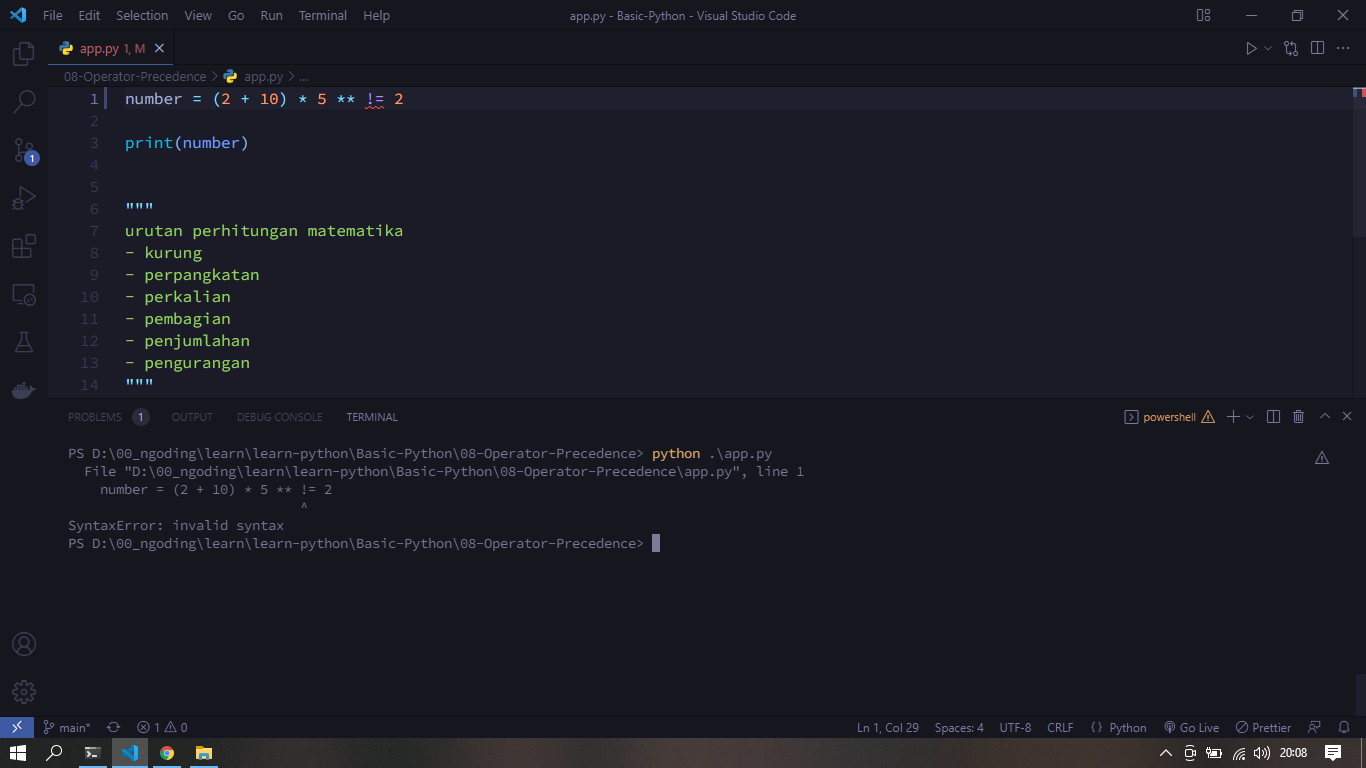
\includegraphics[width=0.5\textwidth]{gambar/09_error.png}
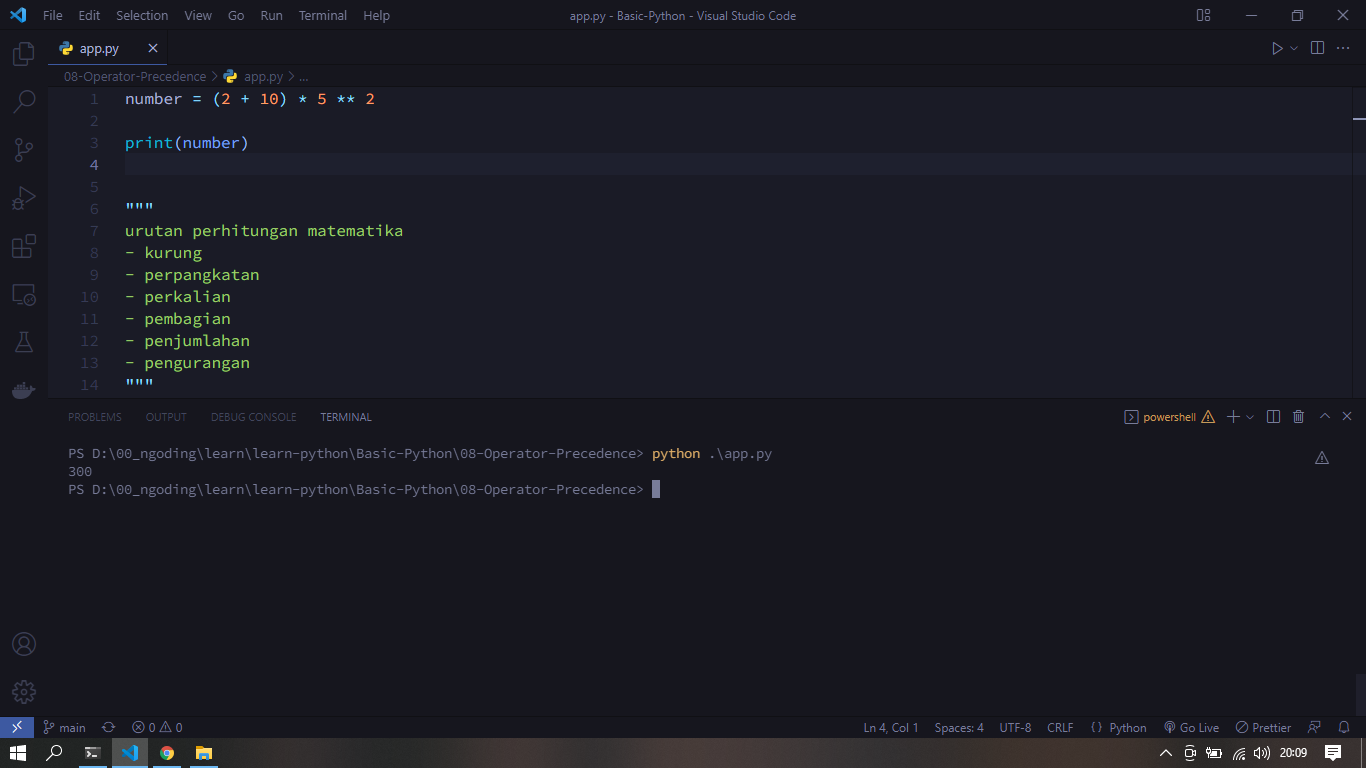
\includegraphics[width=0.5\textwidth]{gambar/09_penanganan.png}

\section{Error 2 dan penyelesaian}
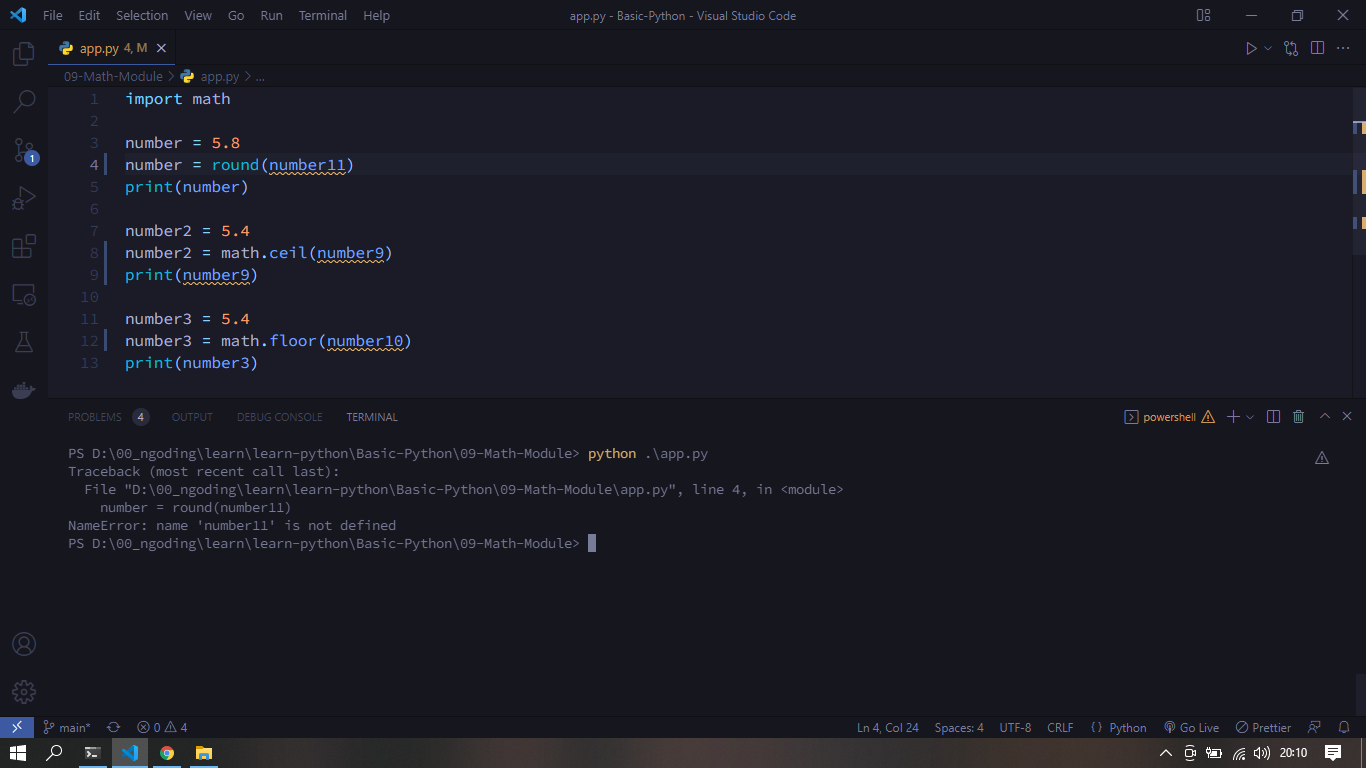
\includegraphics[width=0.5\textwidth]{gambar/10_error.png}
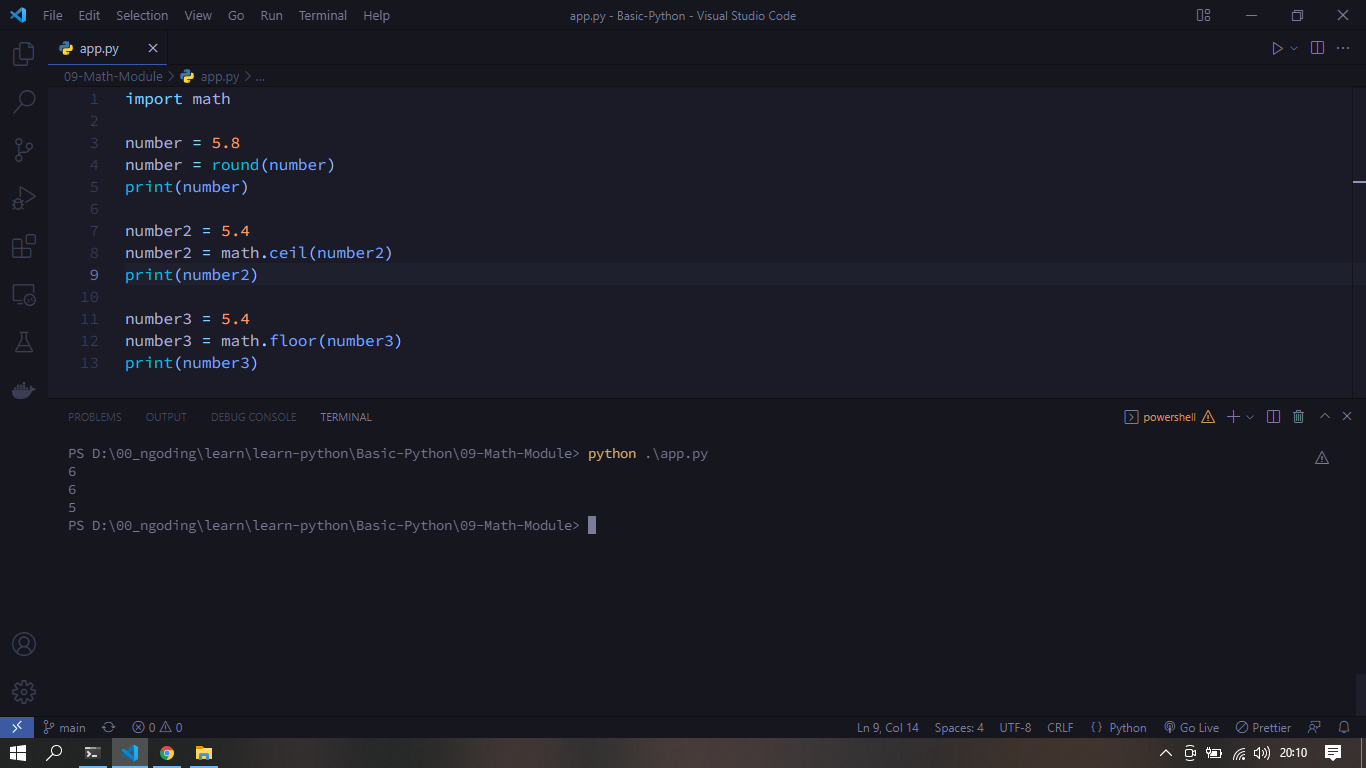
\includegraphics[width=0.5\textwidth]{gambar/10_penanganan.png}

\section{Error 3 dan penyelesaian}
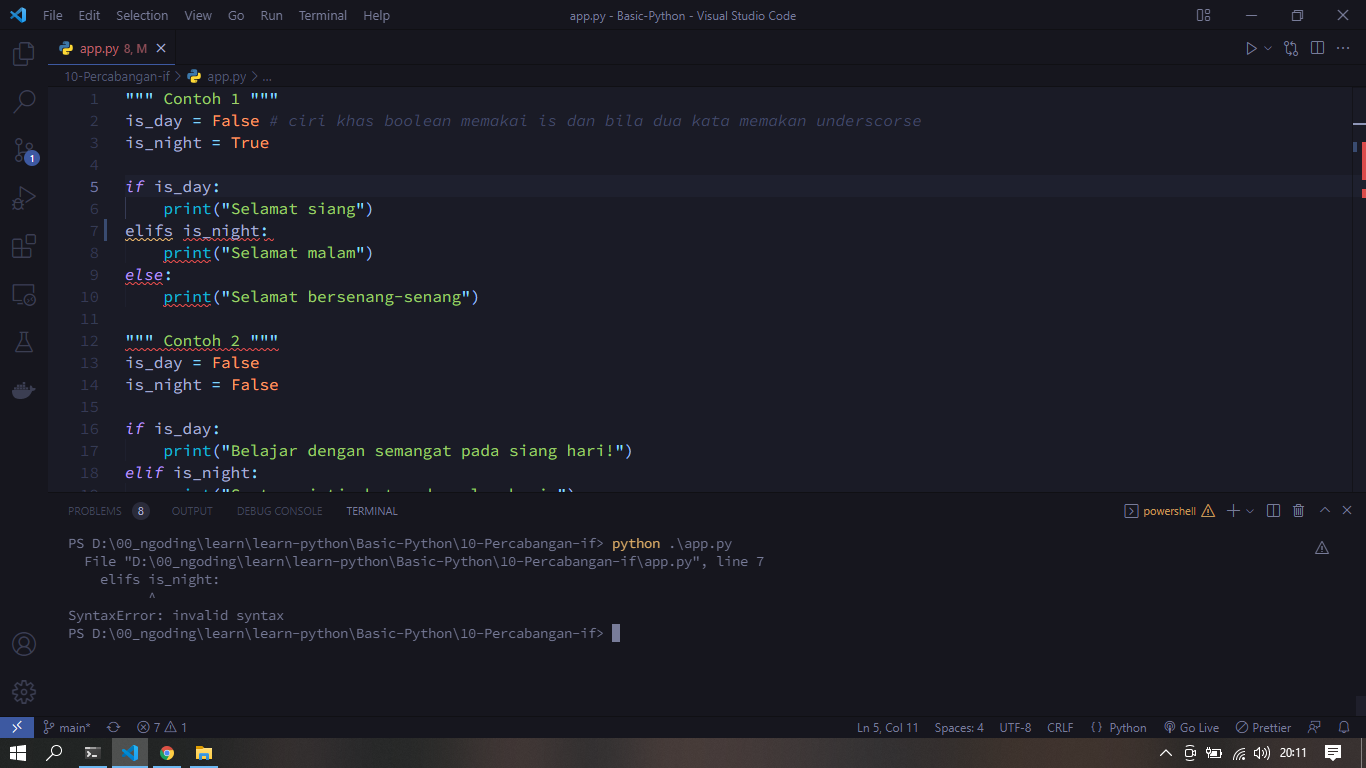
\includegraphics[width=0.5\textwidth]{gambar/11_error.png}
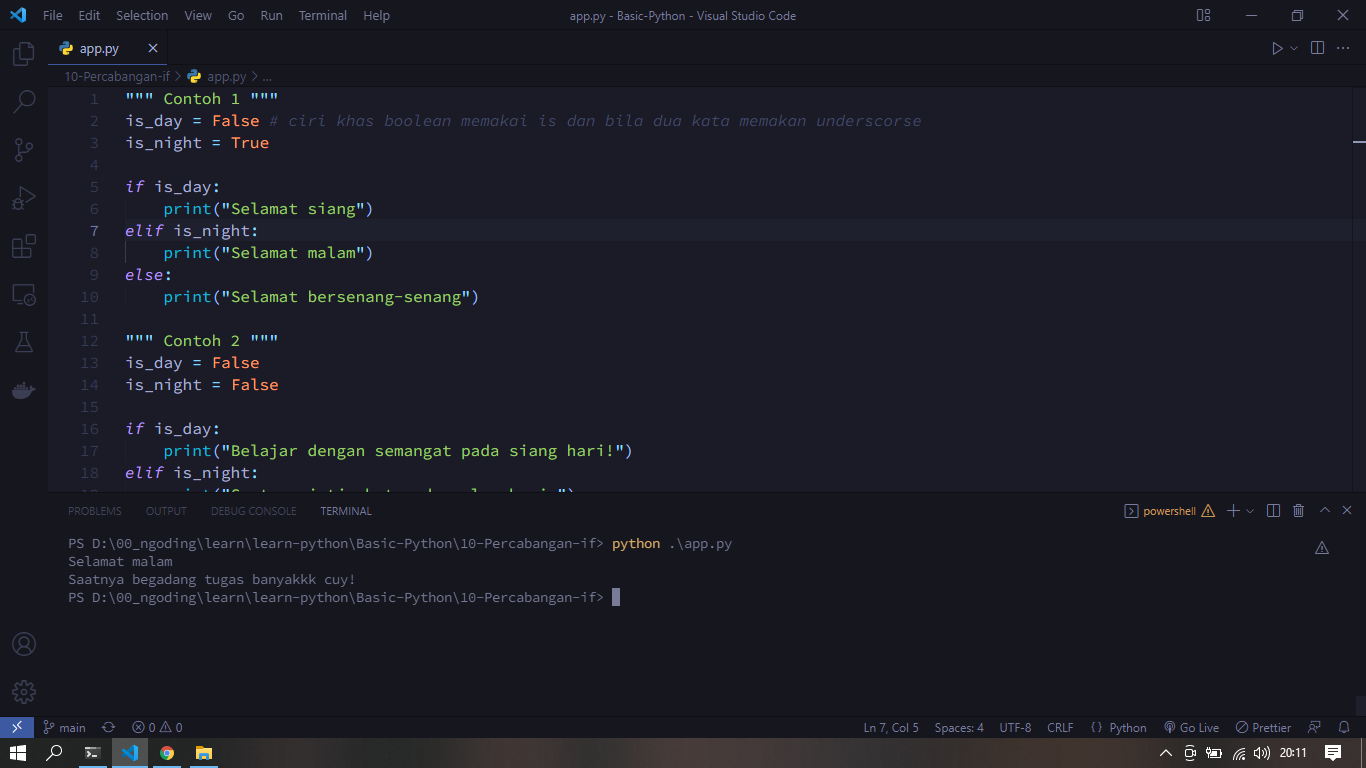
\includegraphics[width=0.5\textwidth]{gambar/11_penanganan.png}

\section{Error 4 dan penyelesaian}
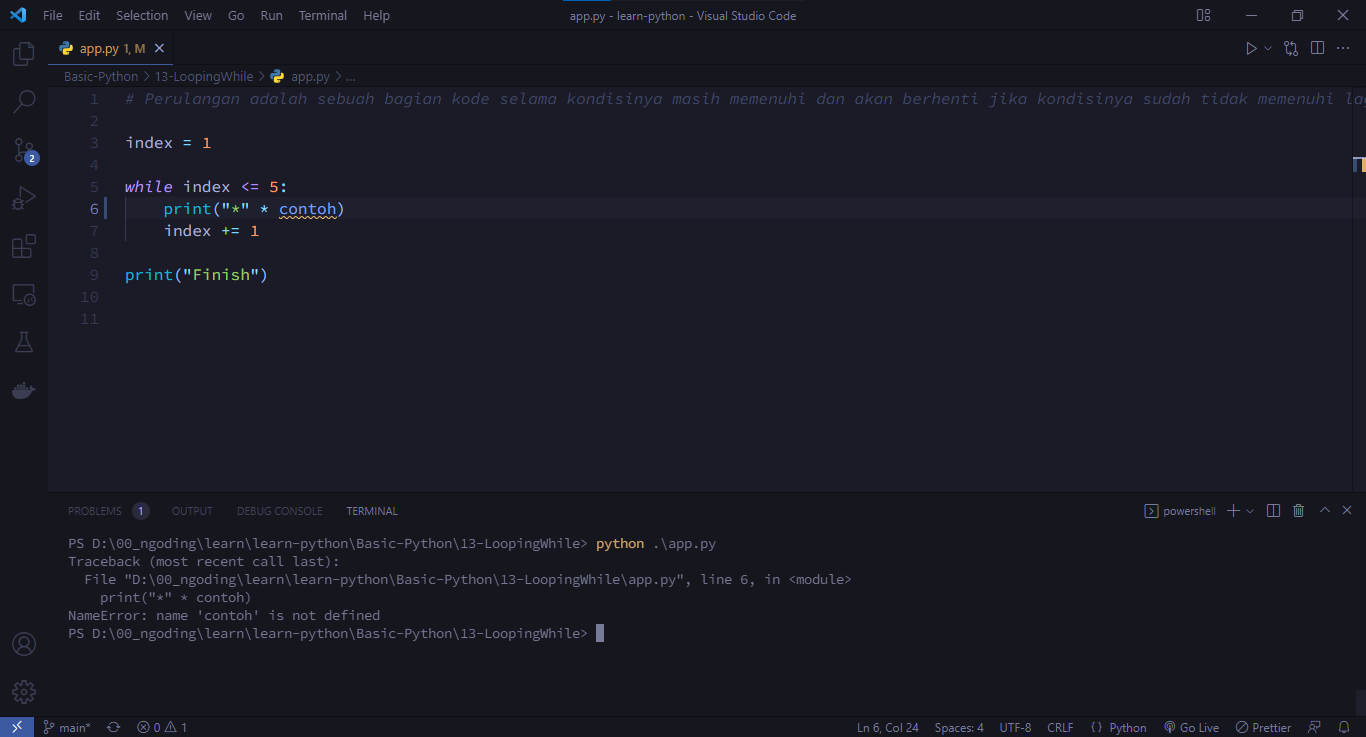
\includegraphics[width=0.5\textwidth]{gambar/13_error.png}
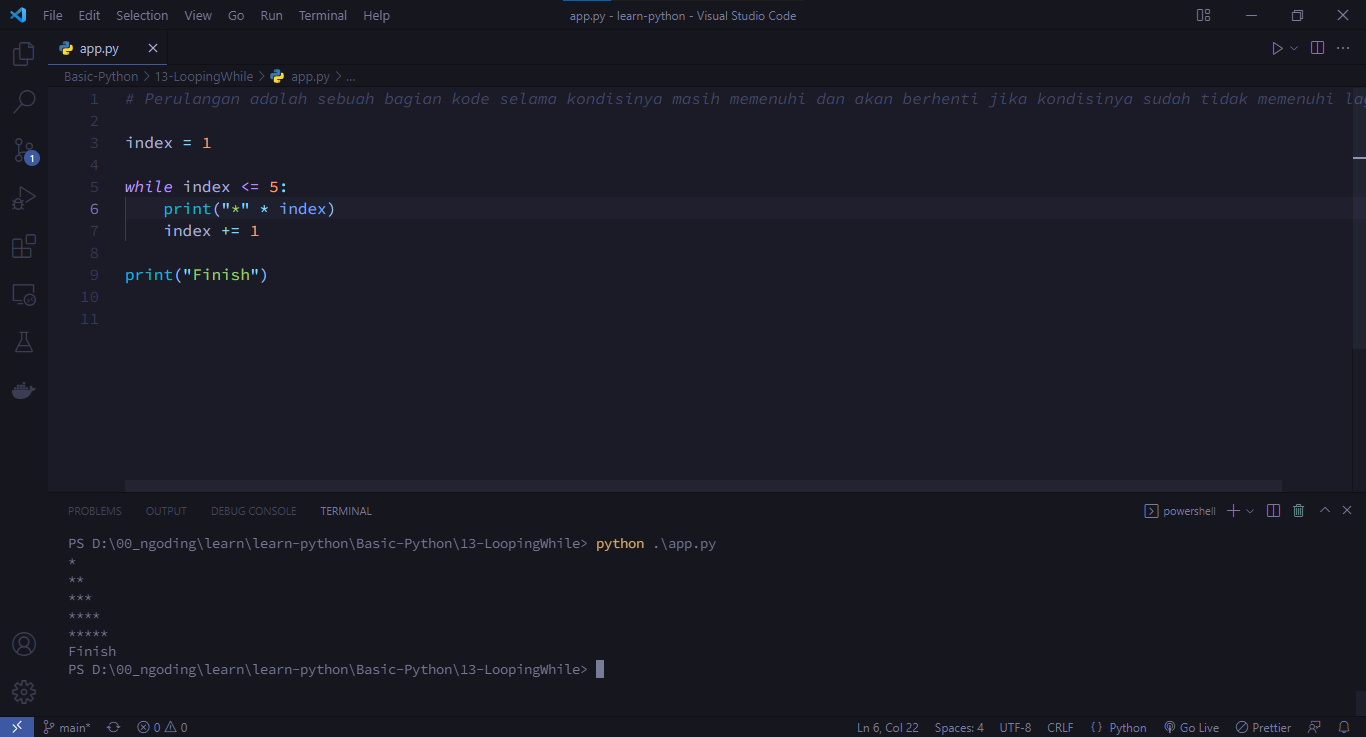
\includegraphics[width=0.5\textwidth]{gambar/13_penanganan.png}

\section{Error 5 dan penyelesaian}
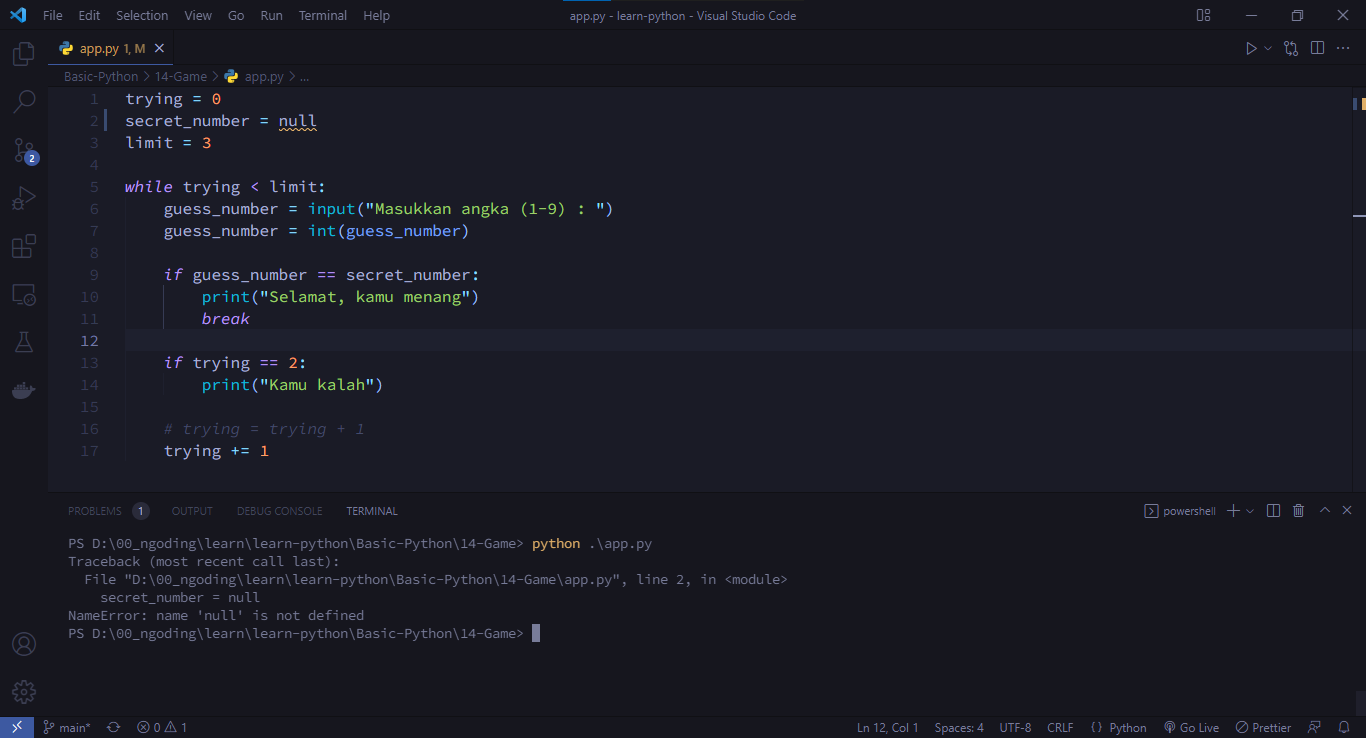
\includegraphics[width=0.5\textwidth]{gambar/14_error.png}
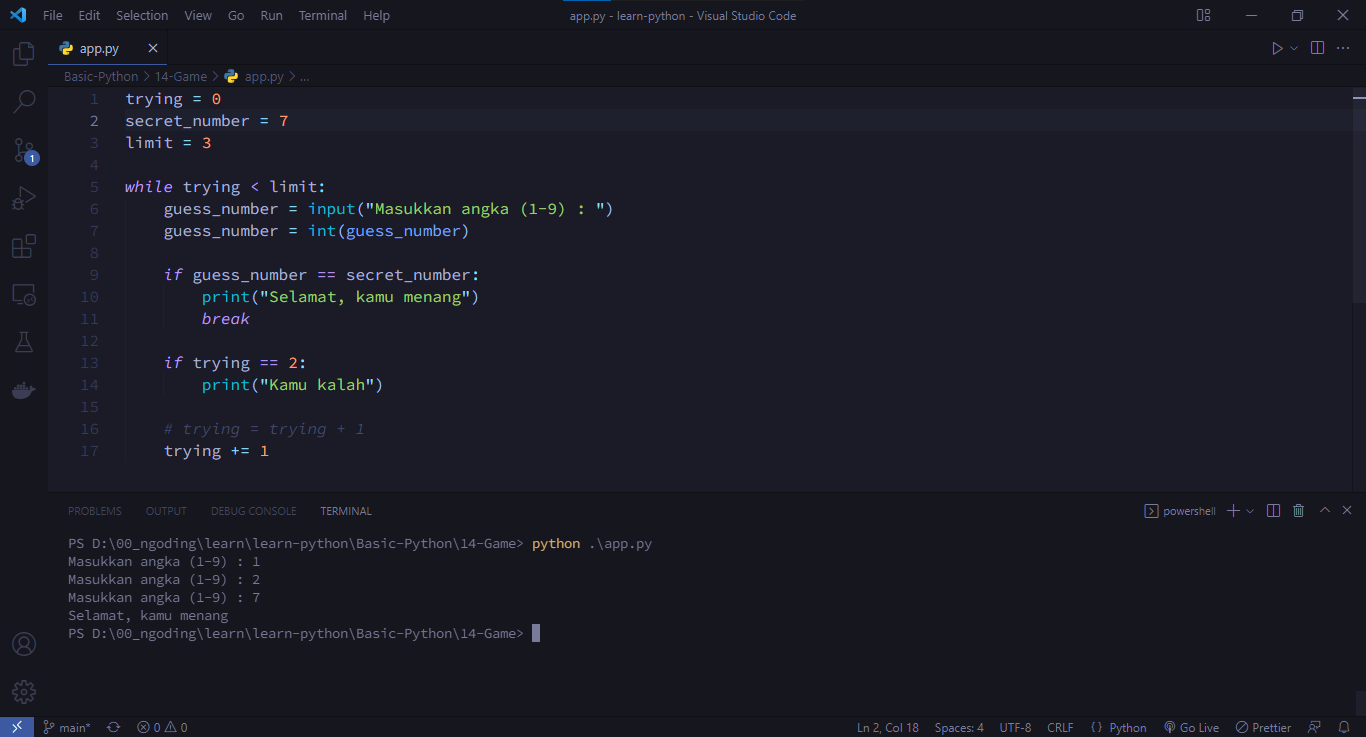
\includegraphics[width=0.5\textwidth]{gambar/14_penanganan.png}

\section{Error 6 dan penyelesaian}
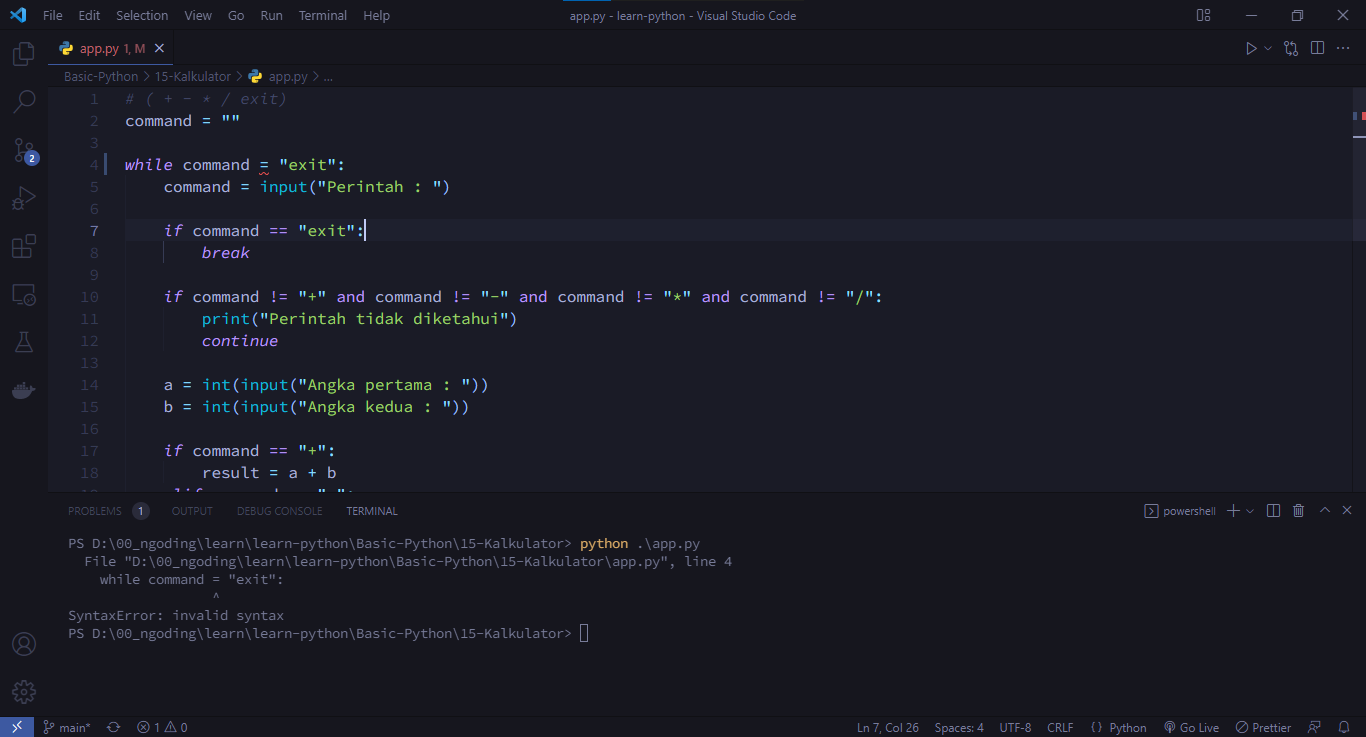
\includegraphics[width=0.5\textwidth]{gambar/15_error.png}
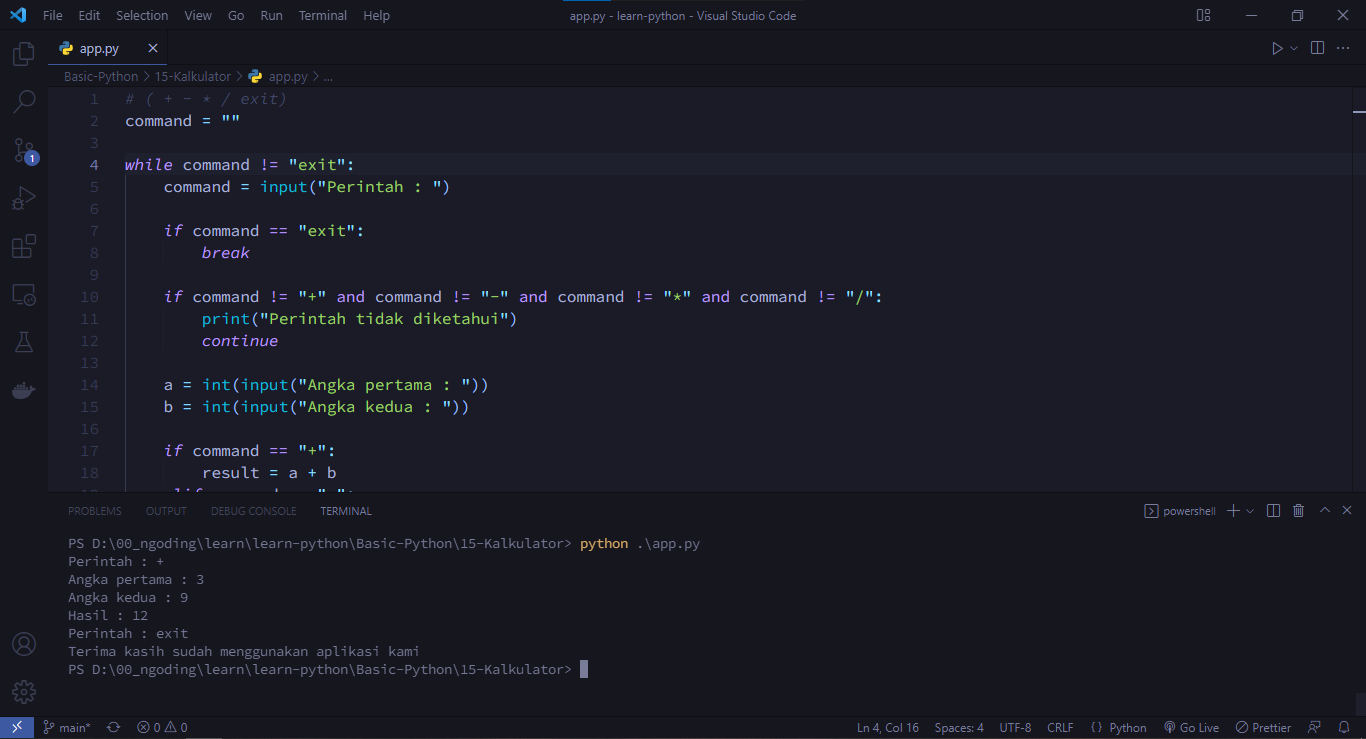
\includegraphics[width=0.5\textwidth]{gambar/15_penanganan.png}

\section{Error 7 dan penyelesaian}
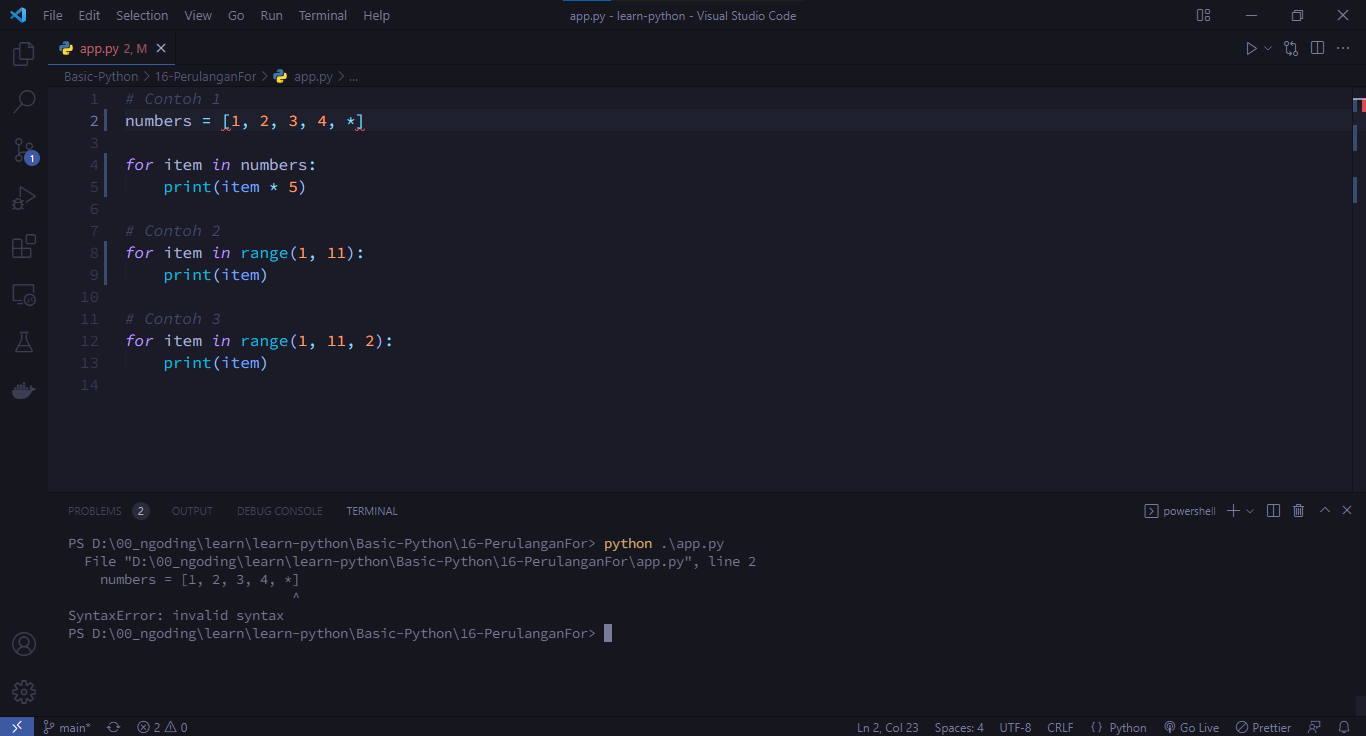
\includegraphics[width=0.5\textwidth]{gambar/16_error.png}
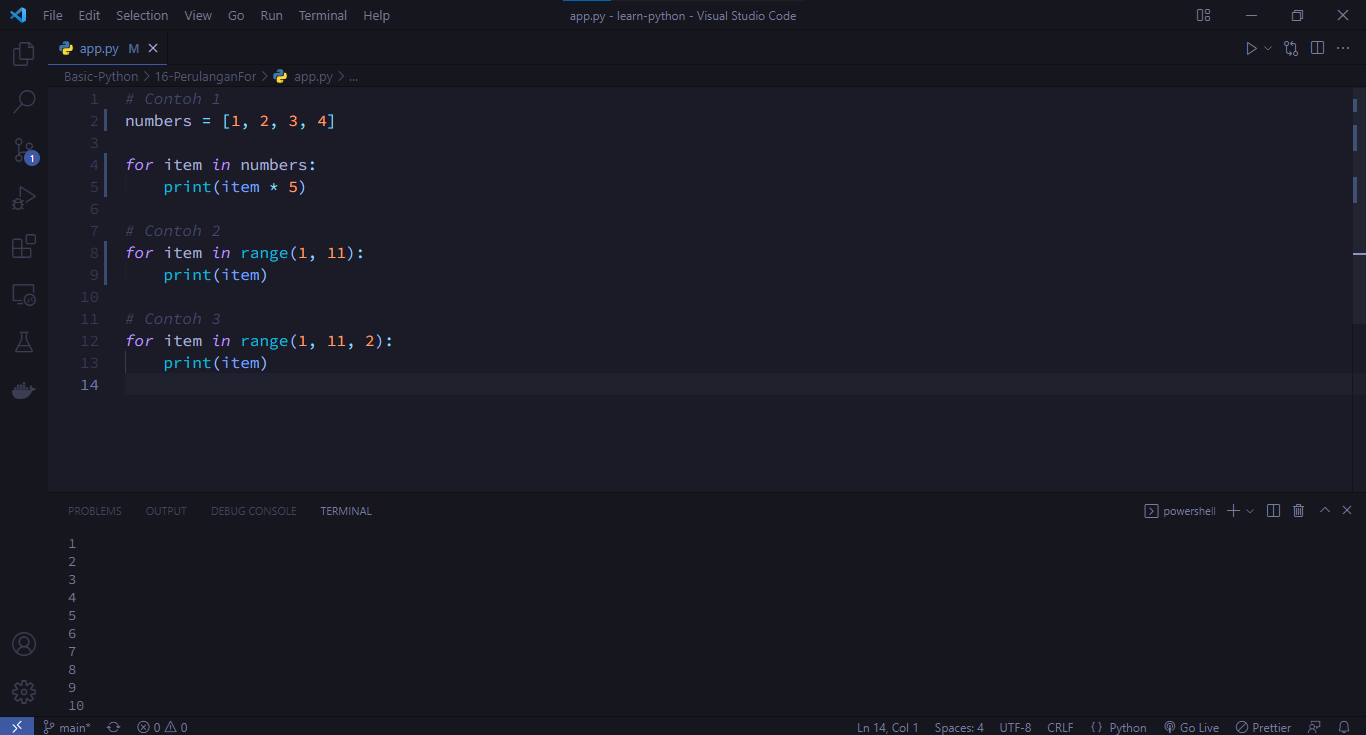
\includegraphics[width=0.5\textwidth]{gambar/16_pengananan.png}

\section{Error 8 dan penyelesaian}
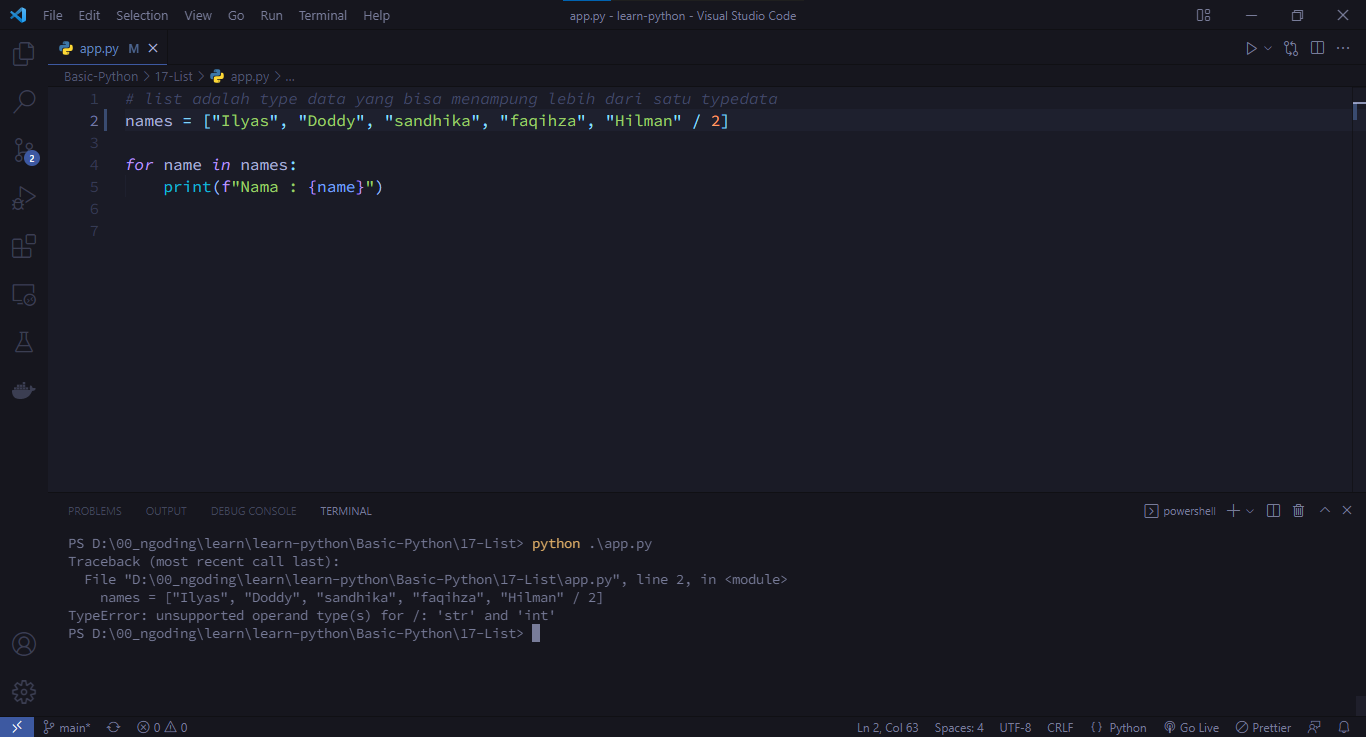
\includegraphics[width=0.5\textwidth]{gambar/17_error.png}
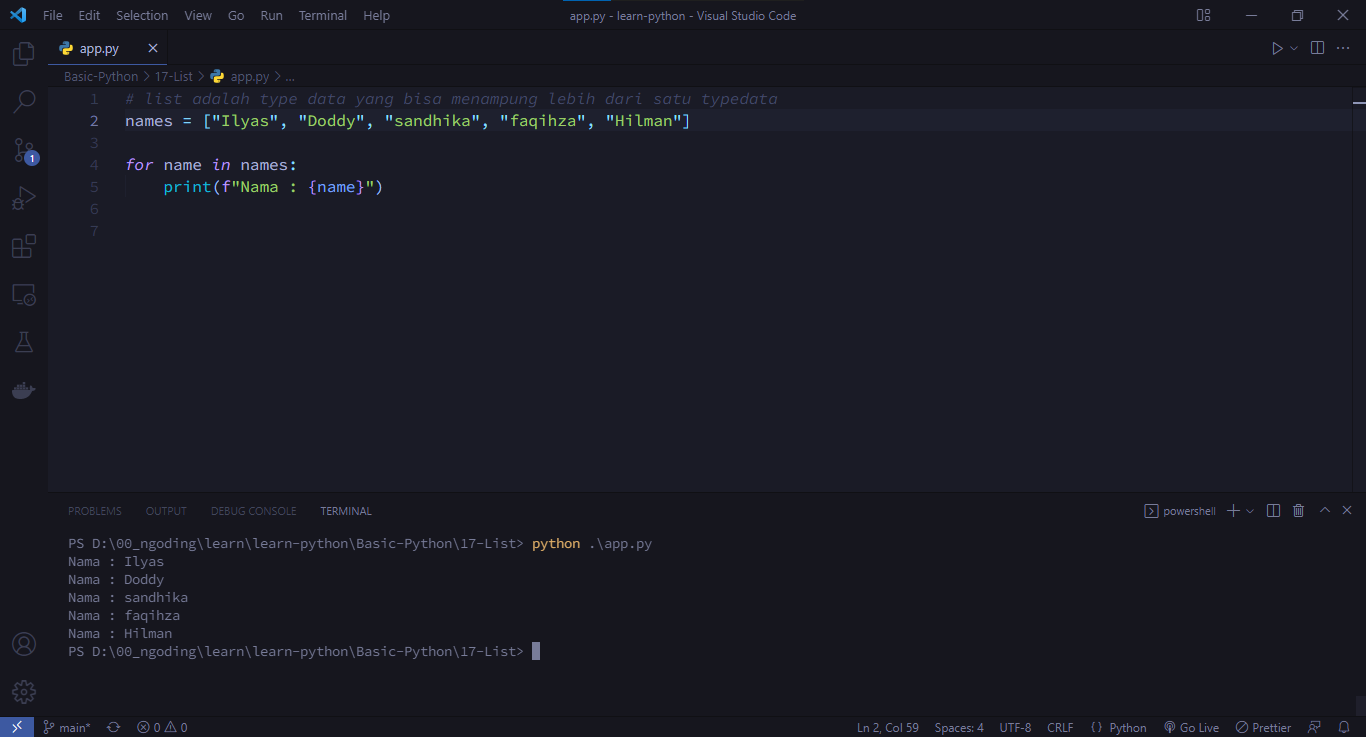
\includegraphics[width=0.5\textwidth]{gambar/17_pengananan.png}

\section{Error 9 dan penyelesaian}
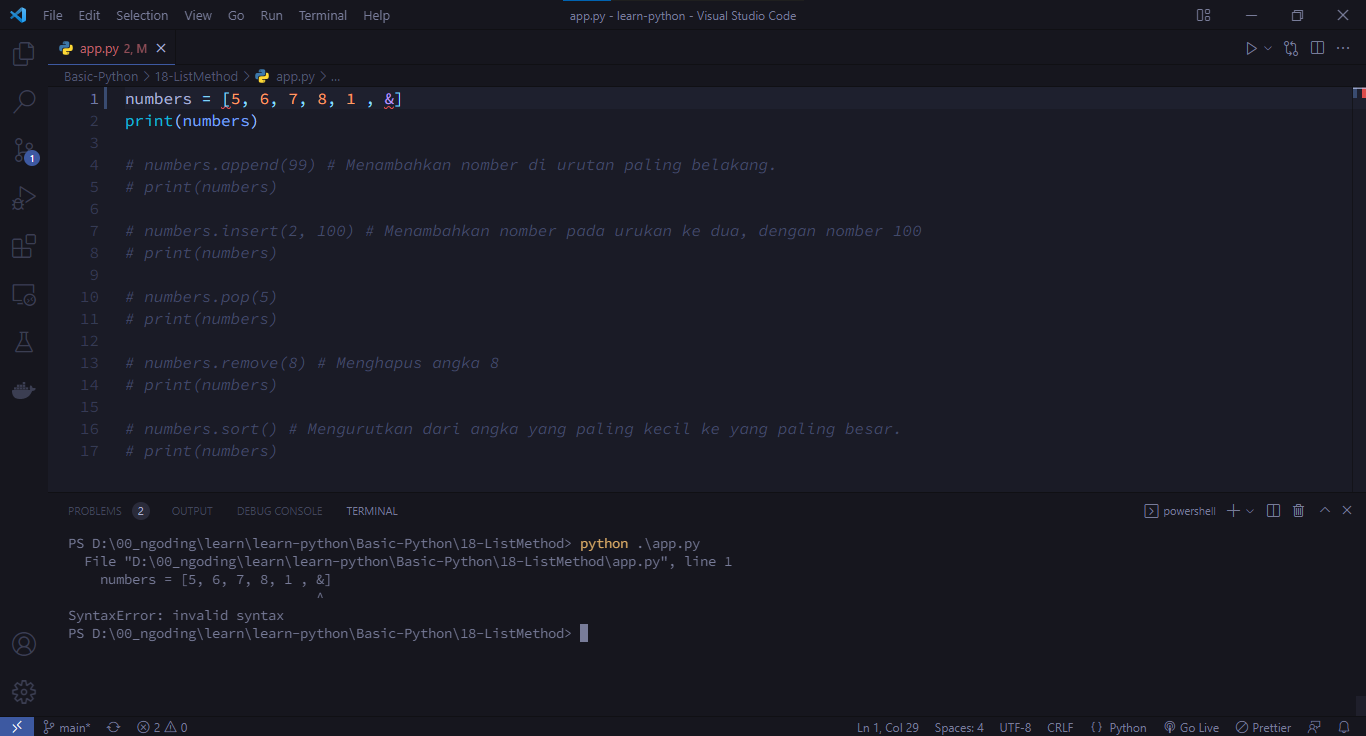
\includegraphics[width=0.5\textwidth]{gambar/18_error.png}
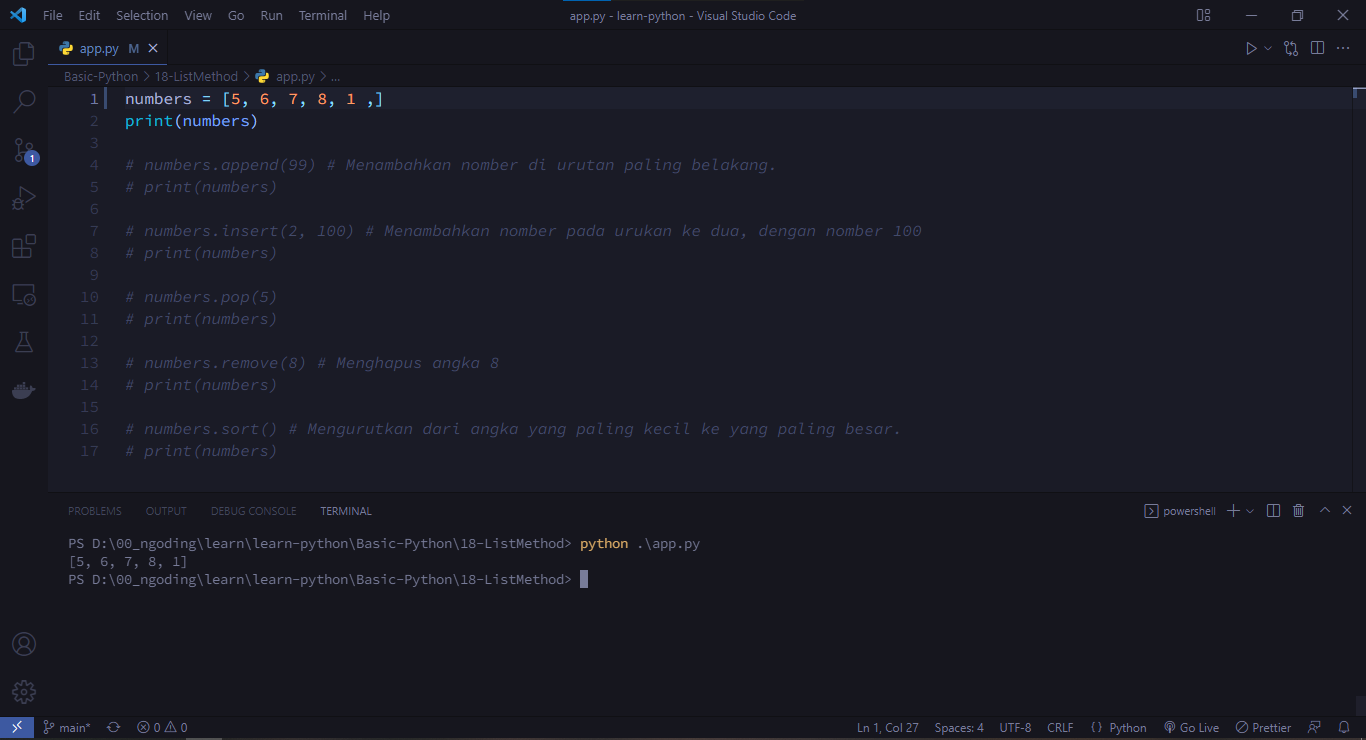
\includegraphics[width=0.5\textwidth]{gambar/18_pengananan.png}

\section{Error 10 dan penyelesaian}
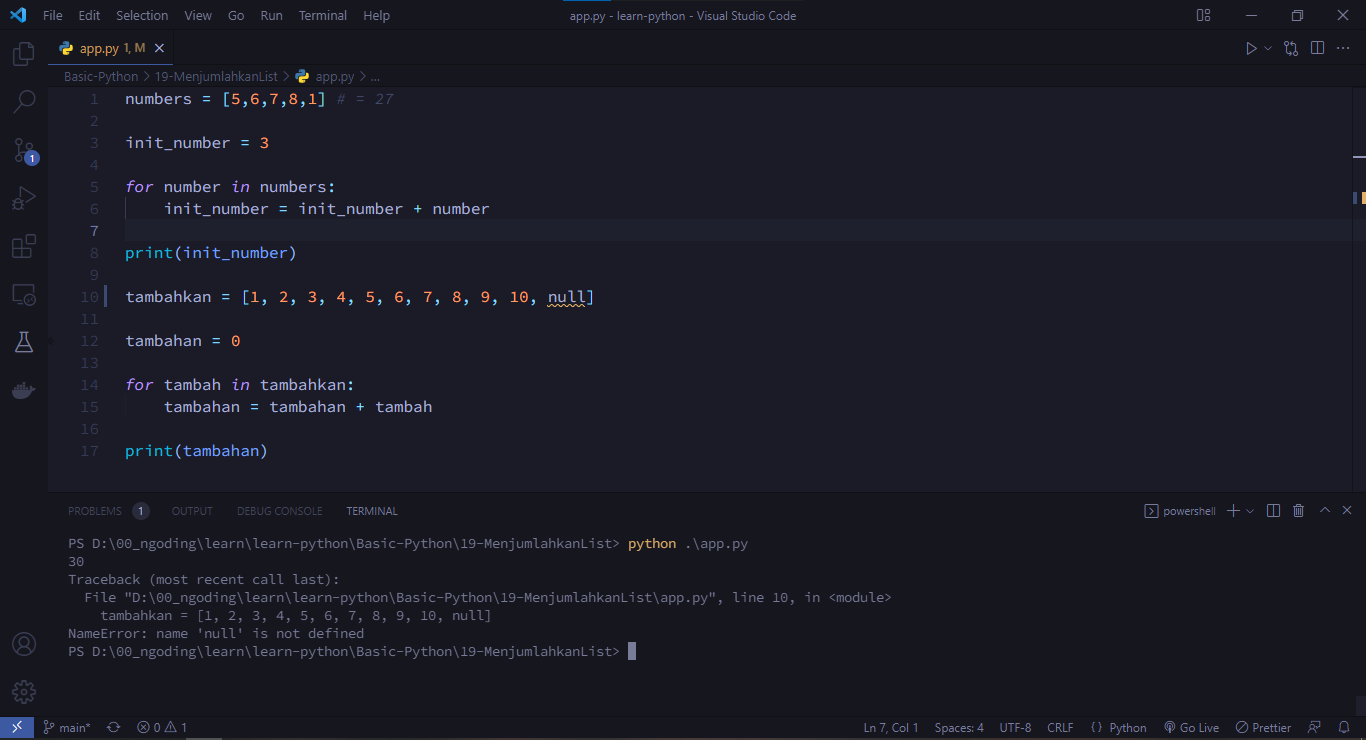
\includegraphics[width=0.5\textwidth]{gambar/19_error.png}
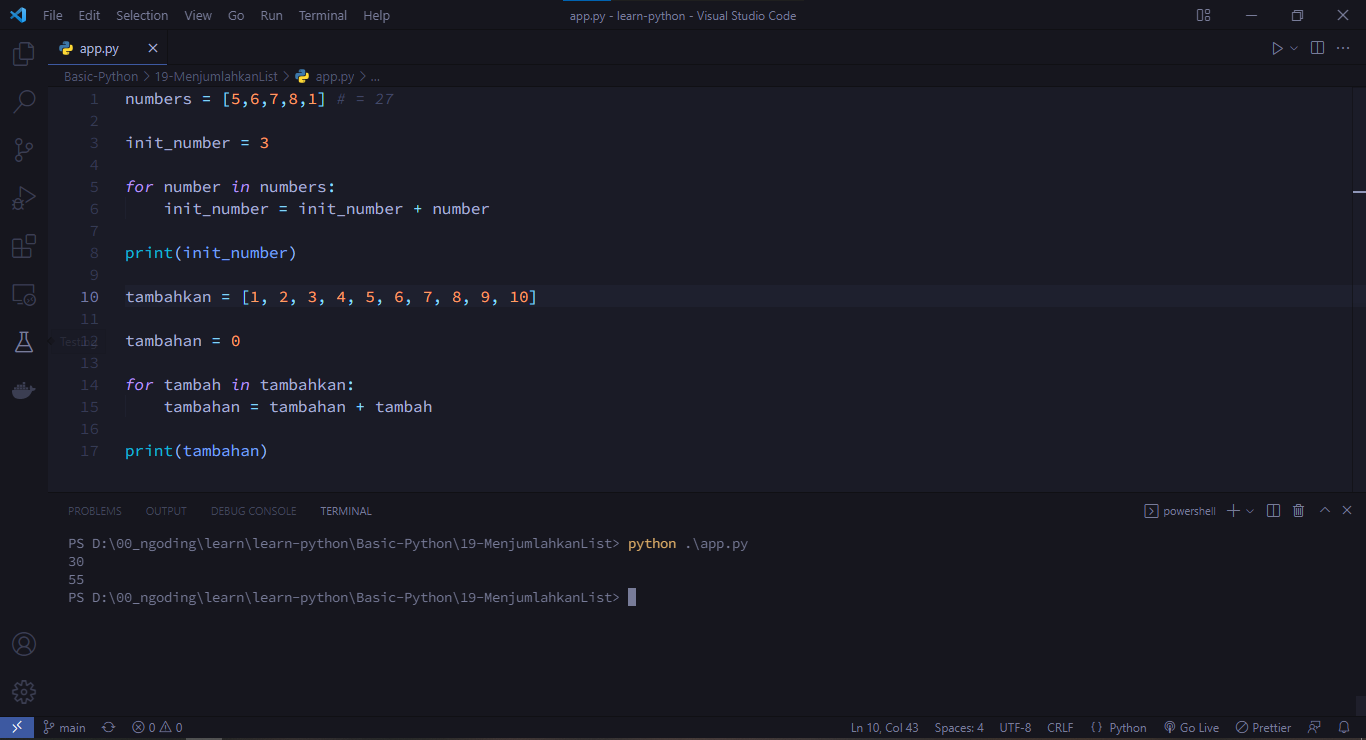
\includegraphics[width=0.5\textwidth]{gambar/19_penanangan.png}

\section{Error 11 dan penyelesaian}
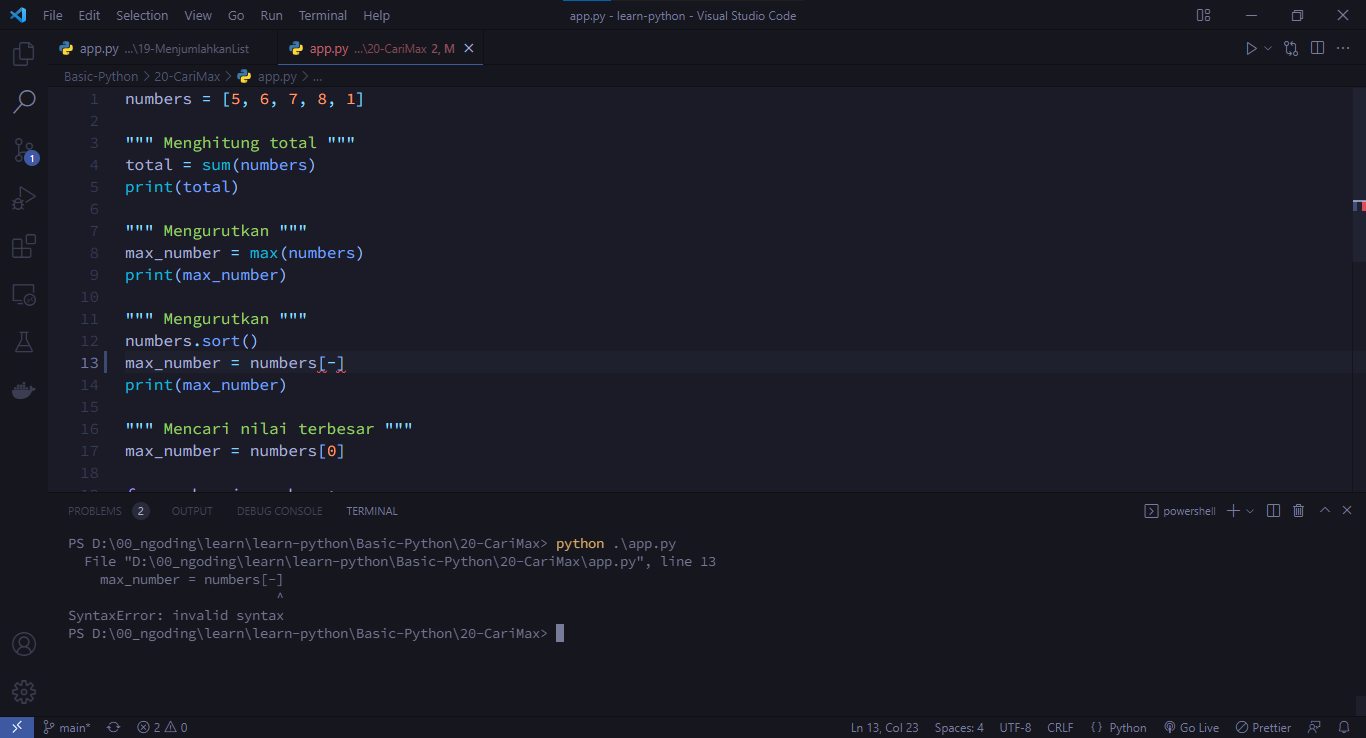
\includegraphics[width=0.5\textwidth]{gambar/20_error.png}
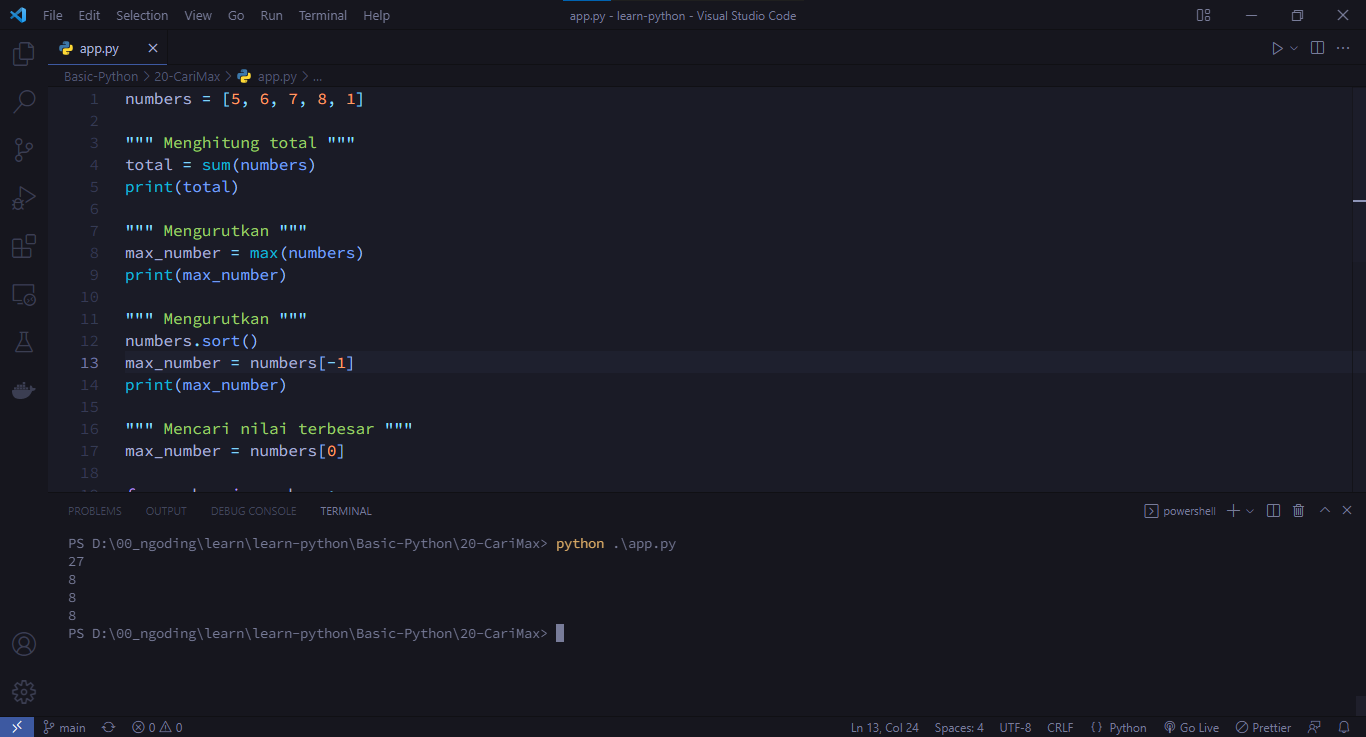
\includegraphics[width=0.5\textwidth]{gambar/20_pengananan.png}

\section{Error 12 dan penyelesaian}
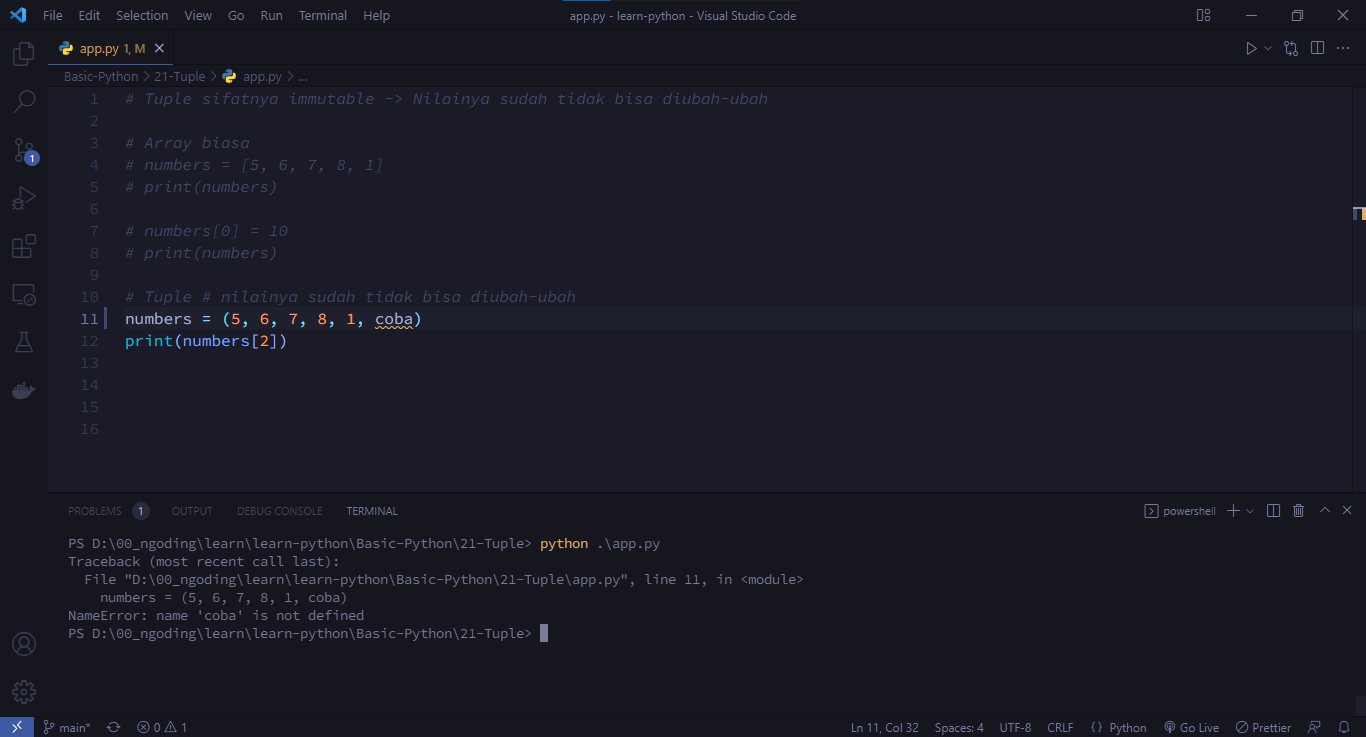
\includegraphics[width=0.5\textwidth]{gambar/21_error.png}
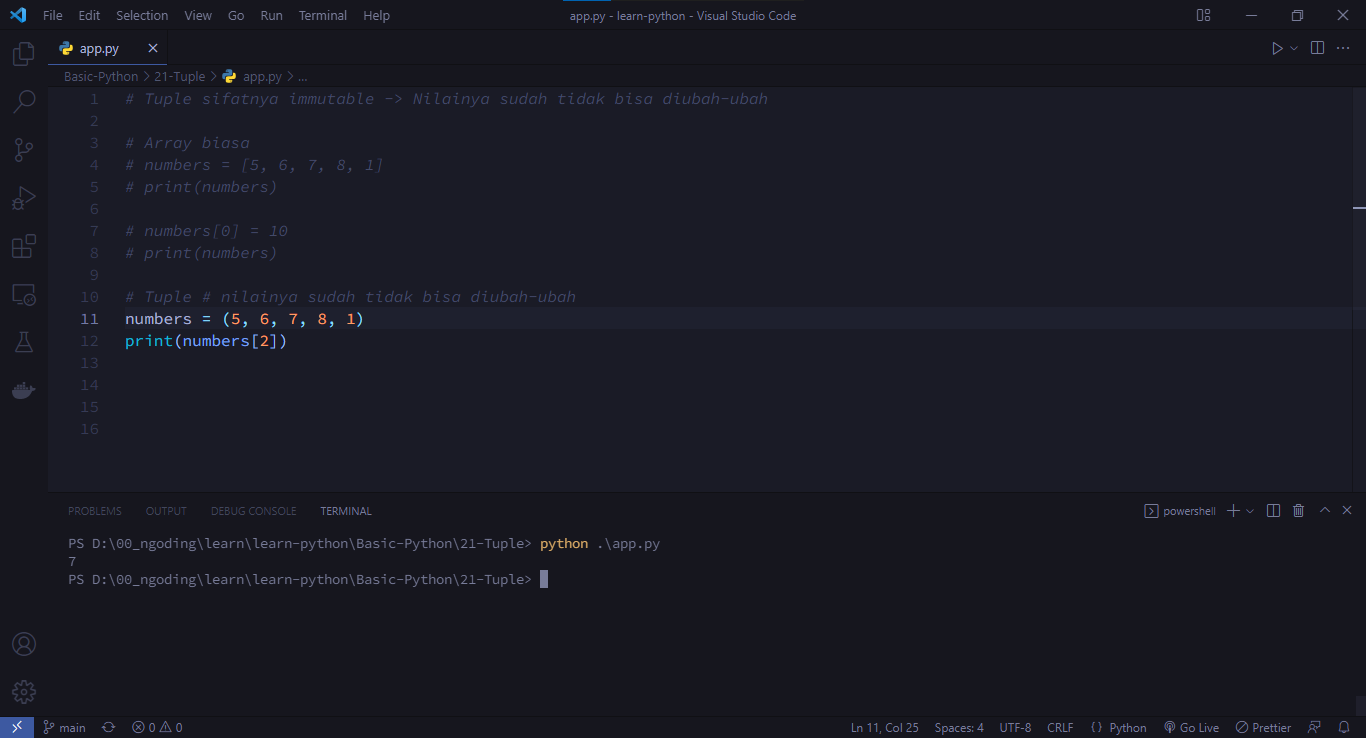
\includegraphics[width=0.5\textwidth]{gambar/21_penanganan.png}

\section{Error 13 dan penyelesaian}
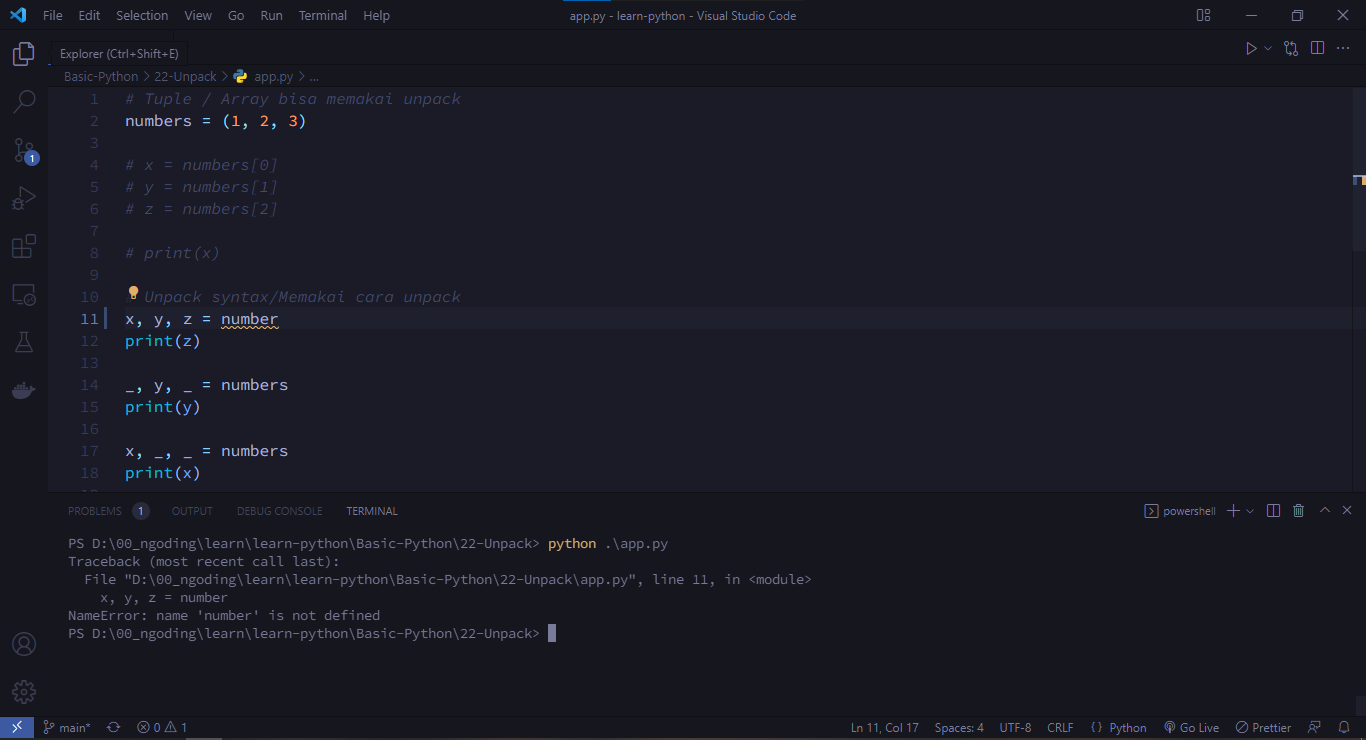
\includegraphics[width=0.5\textwidth]{gambar/22_error.png}
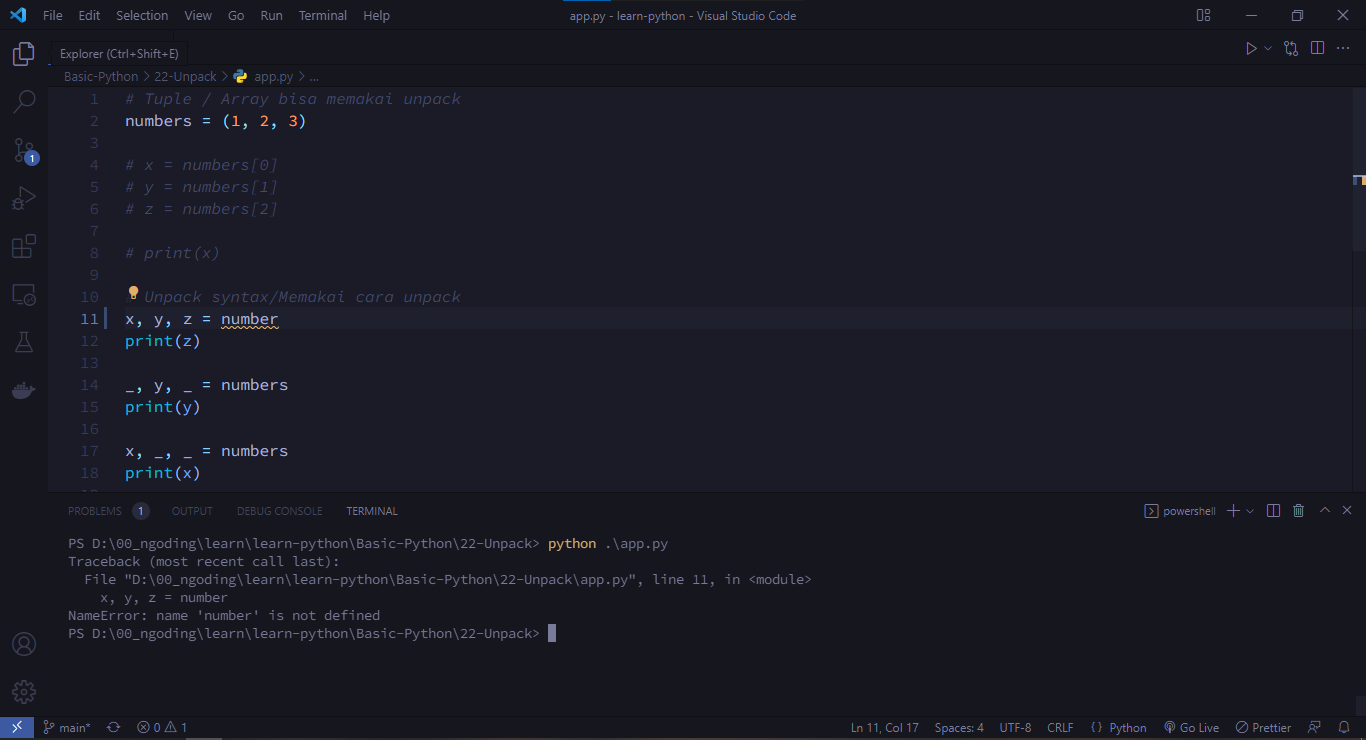
\includegraphics[width=0.5\textwidth]{gambar/22_error.png}

\section{Error 14 dan penyelesaian}
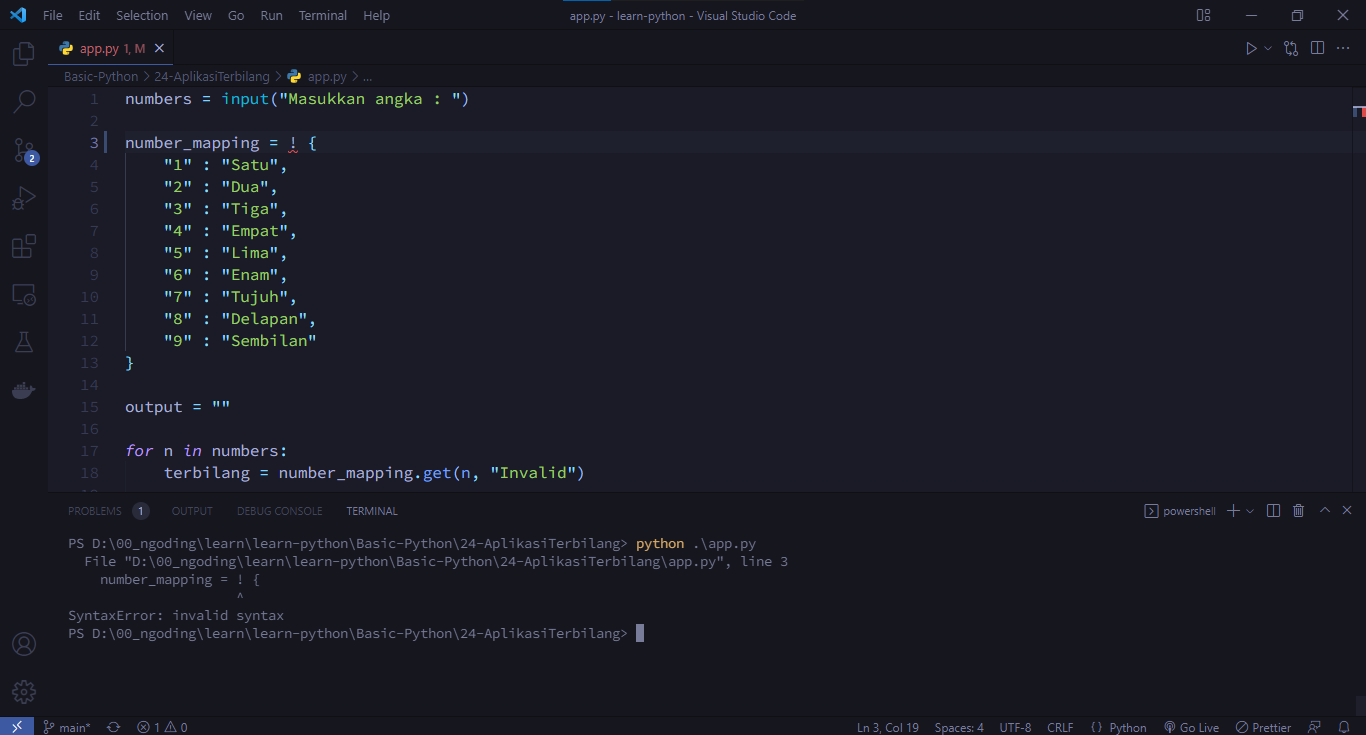
\includegraphics[width=0.5\textwidth]{gambar/24_error.png}
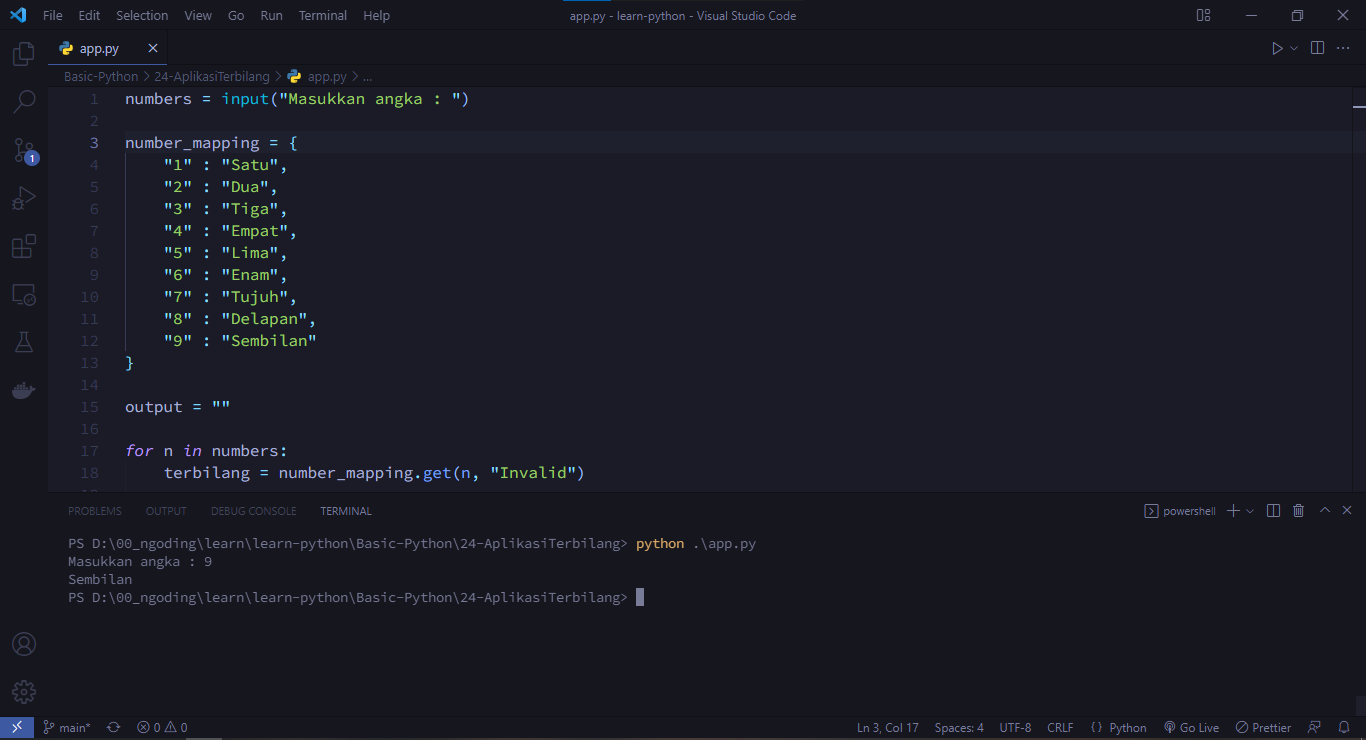
\includegraphics[width=0.5\textwidth]{gambar/24_penanganan.png}

\section{Error 15 dan penyelesaian}
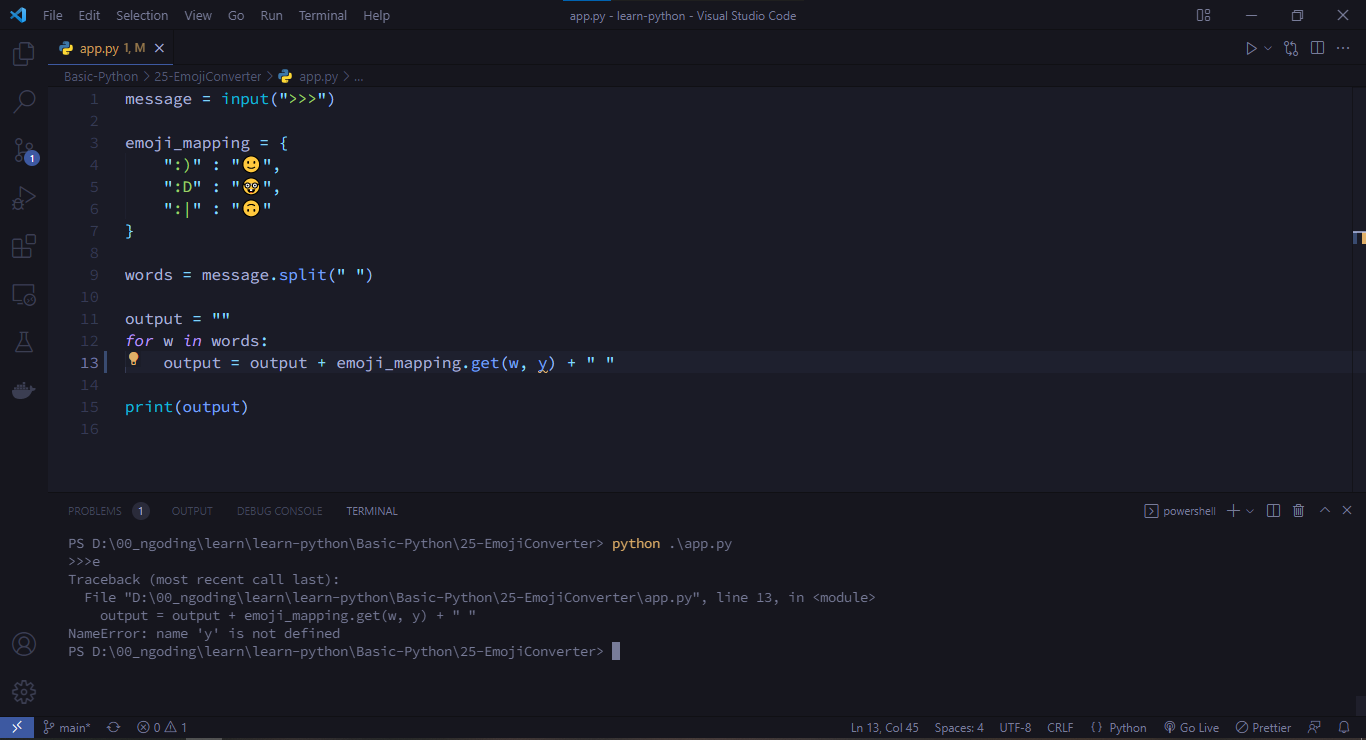
\includegraphics[width=0.5\textwidth]{gambar/25_error.png}
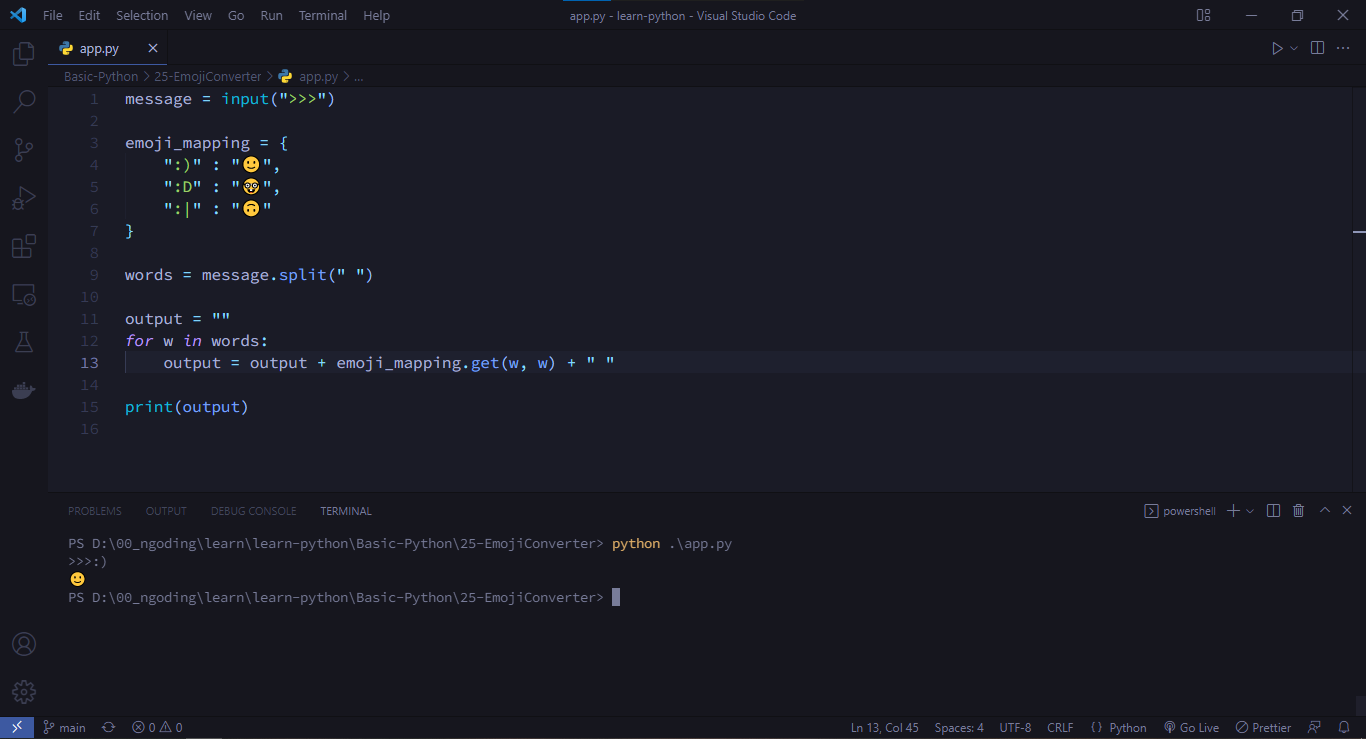
\includegraphics[width=0.5\textwidth]{gambar/25_pengananan.png}

\section{Error 16 dan penyelesaian}
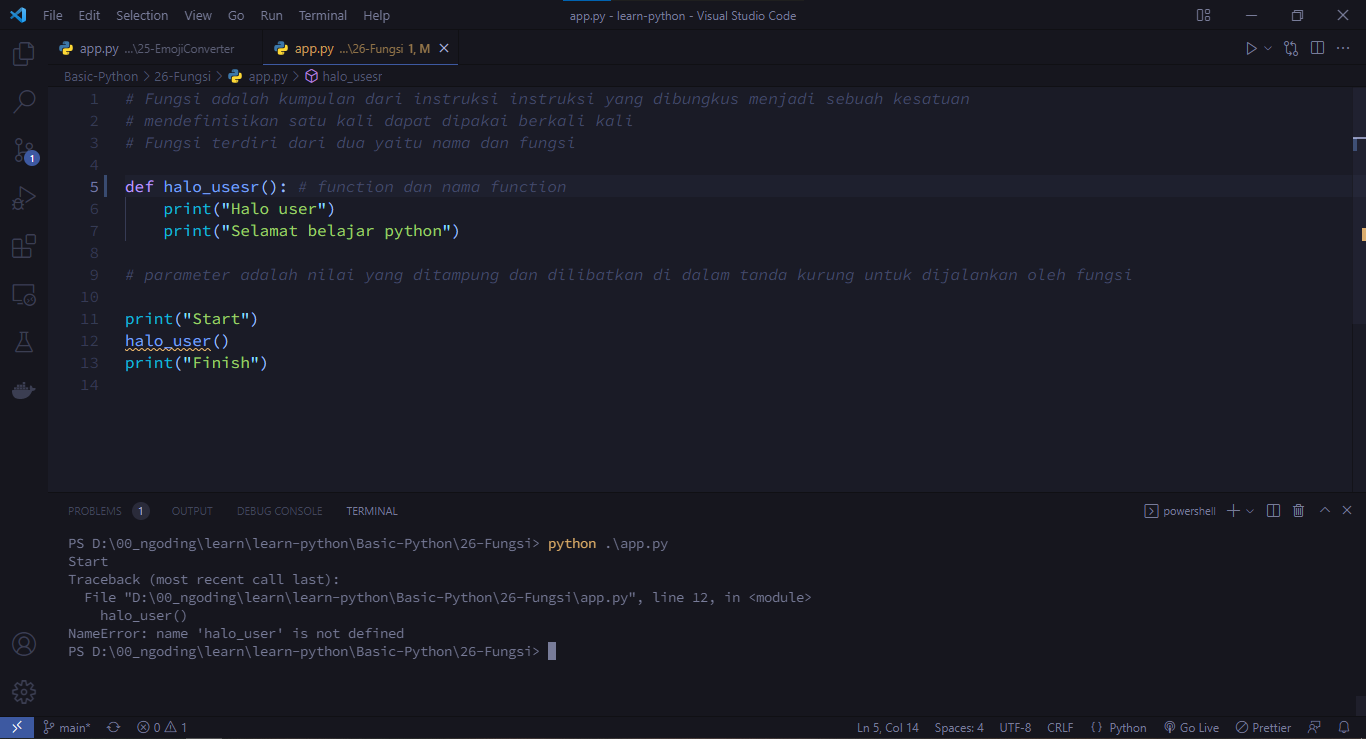
\includegraphics[width=0.5\textwidth]{gambar/26_error.png}
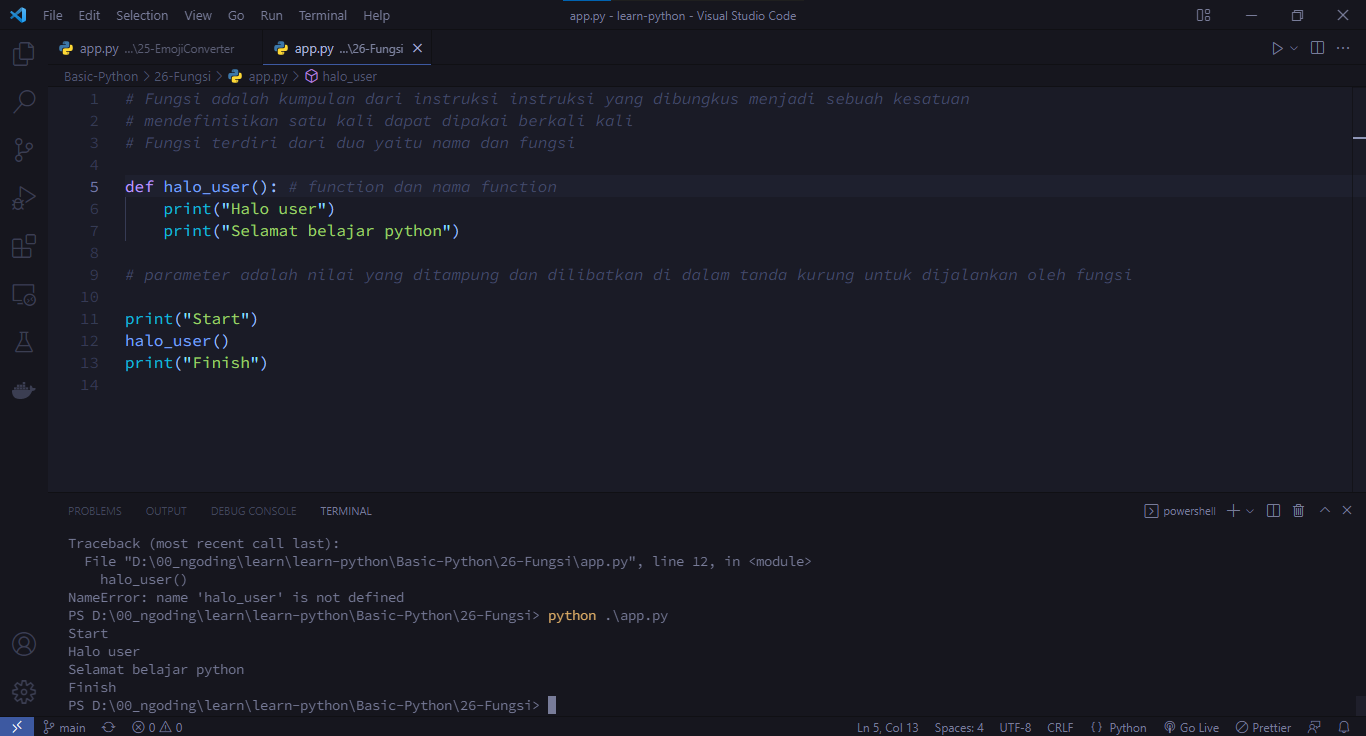
\includegraphics[width=0.5\textwidth]{gambar/26_pengananan.png}

\section{Error 17 dan penyelesaian}
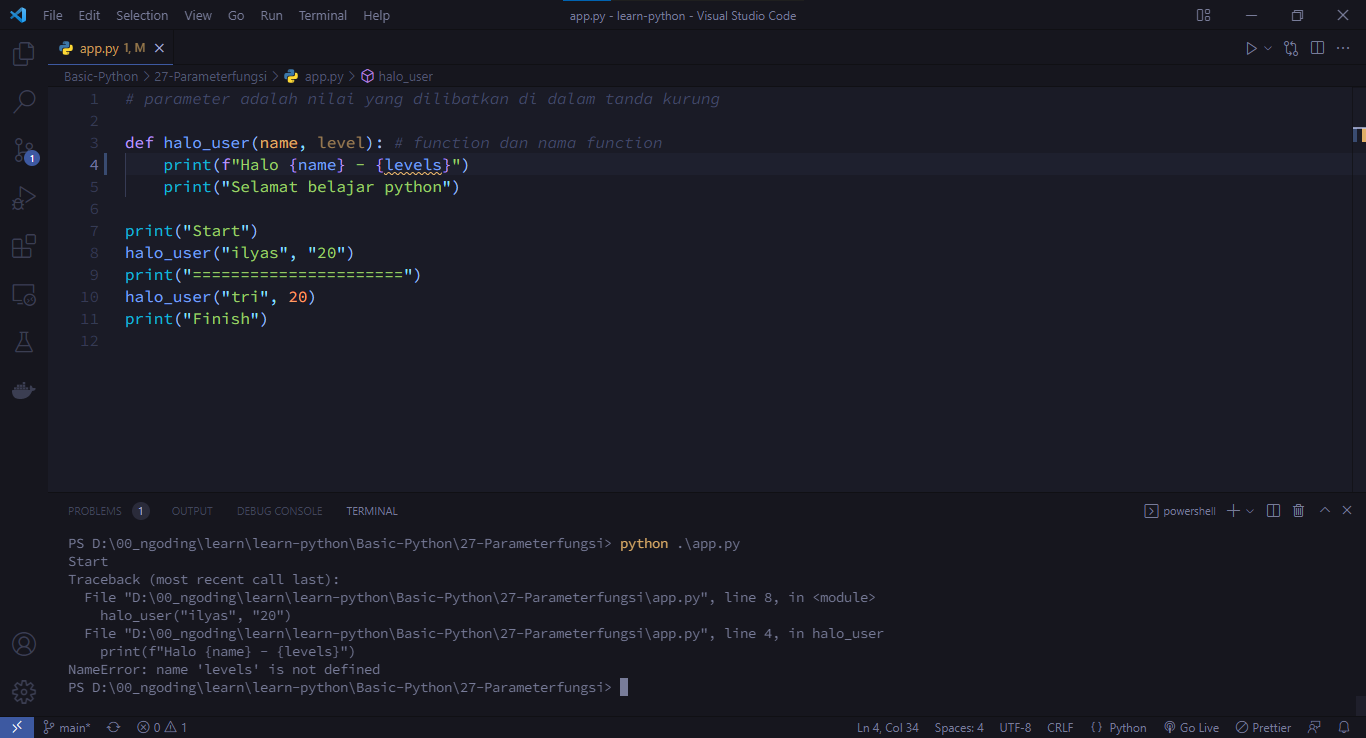
\includegraphics[width=0.5\textwidth]{gambar/27_error.png}
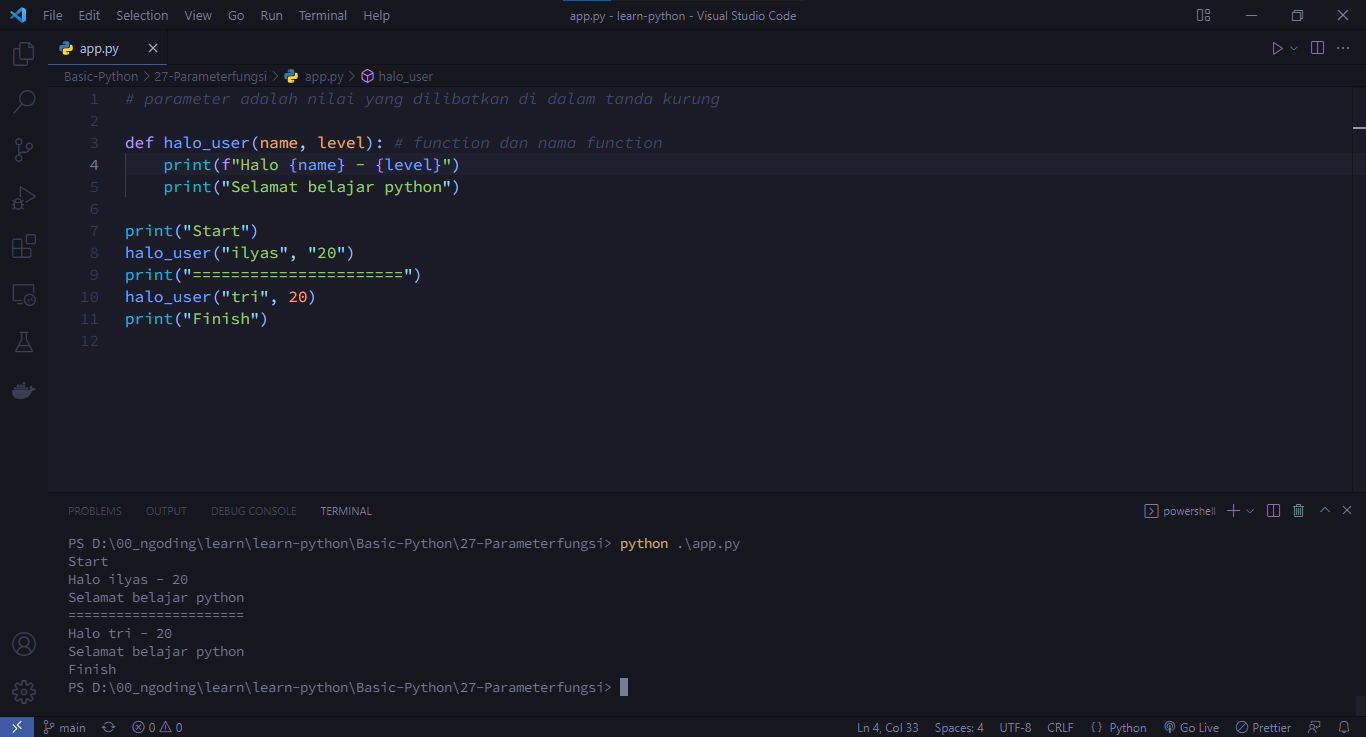
\includegraphics[width=0.5\textwidth]{gambar/27_pengananan.png}

\section{Error 18 dan penyelesaian}
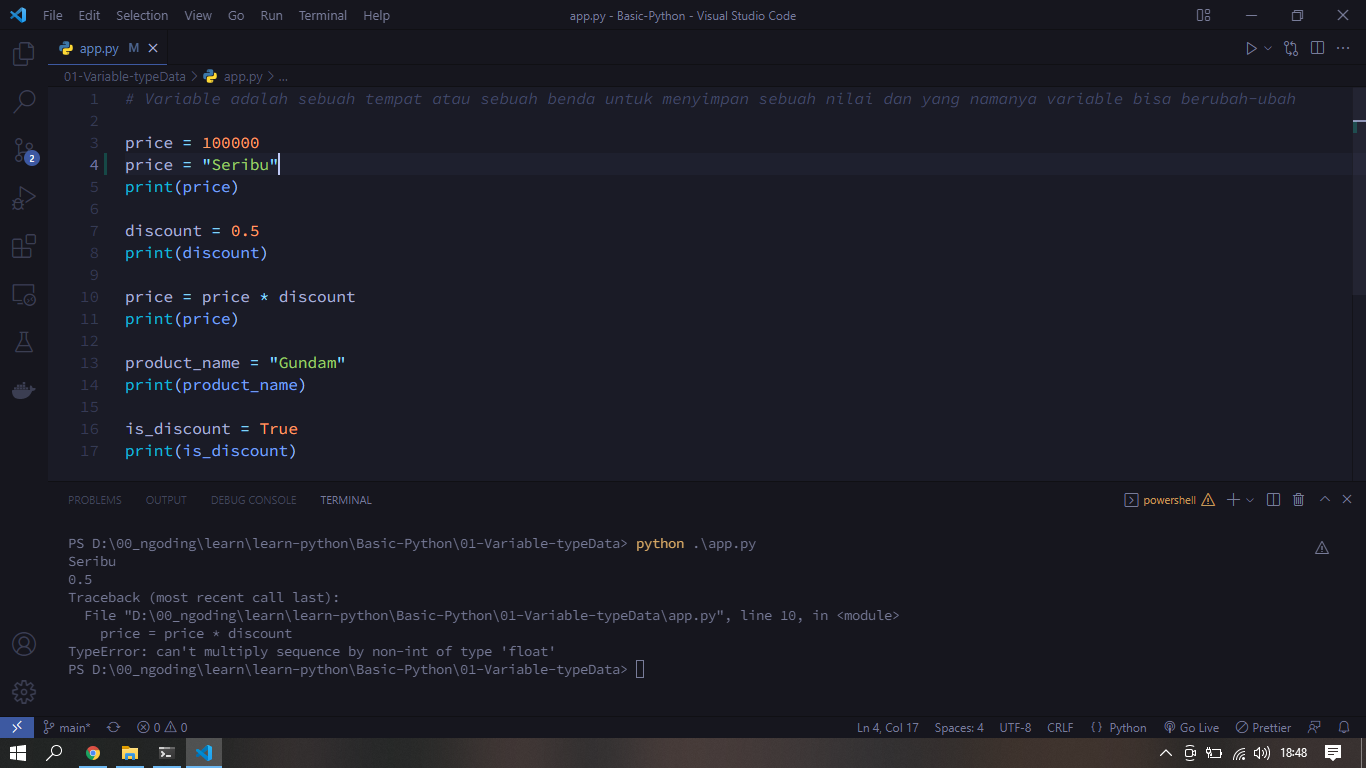
\includegraphics[width=0.5\textwidth]{gambar/02_error.png}
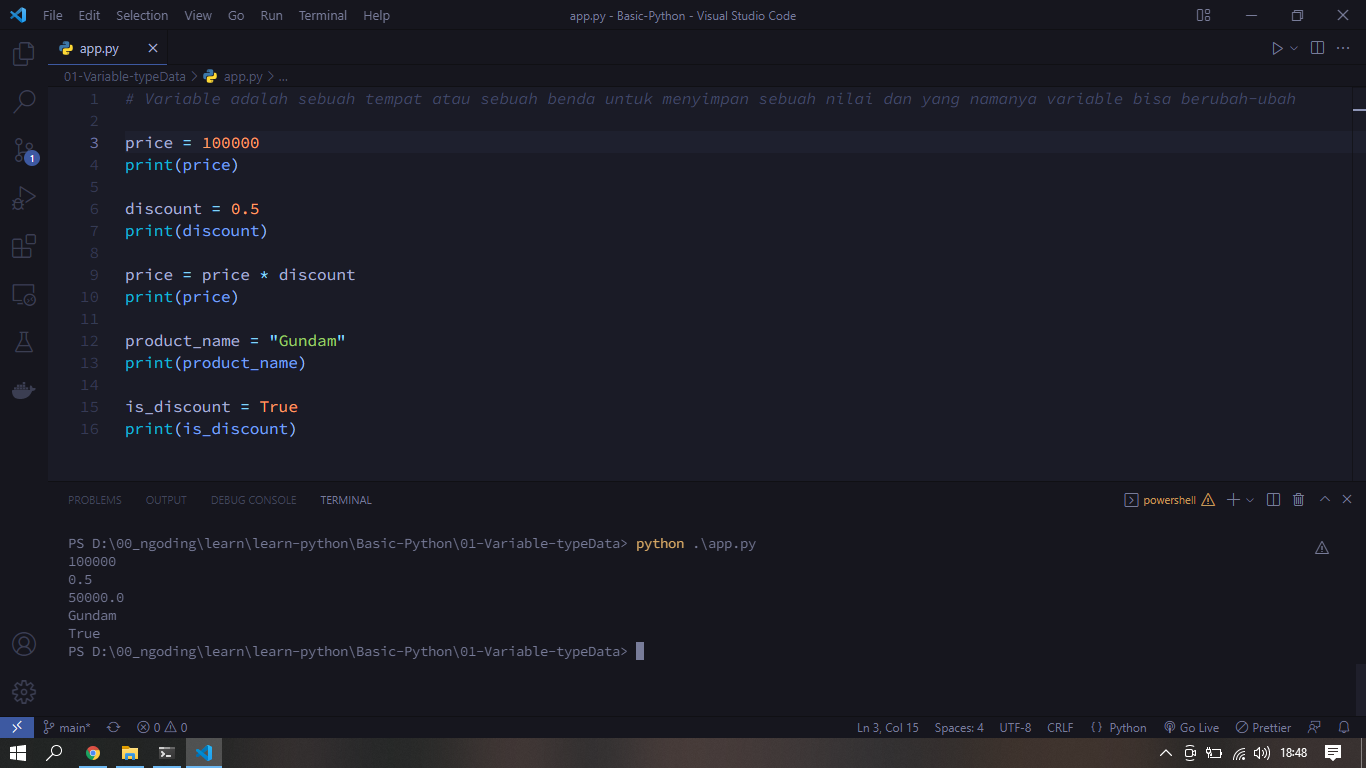
\includegraphics[width=0.5\textwidth]{gambar/02_penanganan.png}

\section{Error 19 dan penyelesaian}
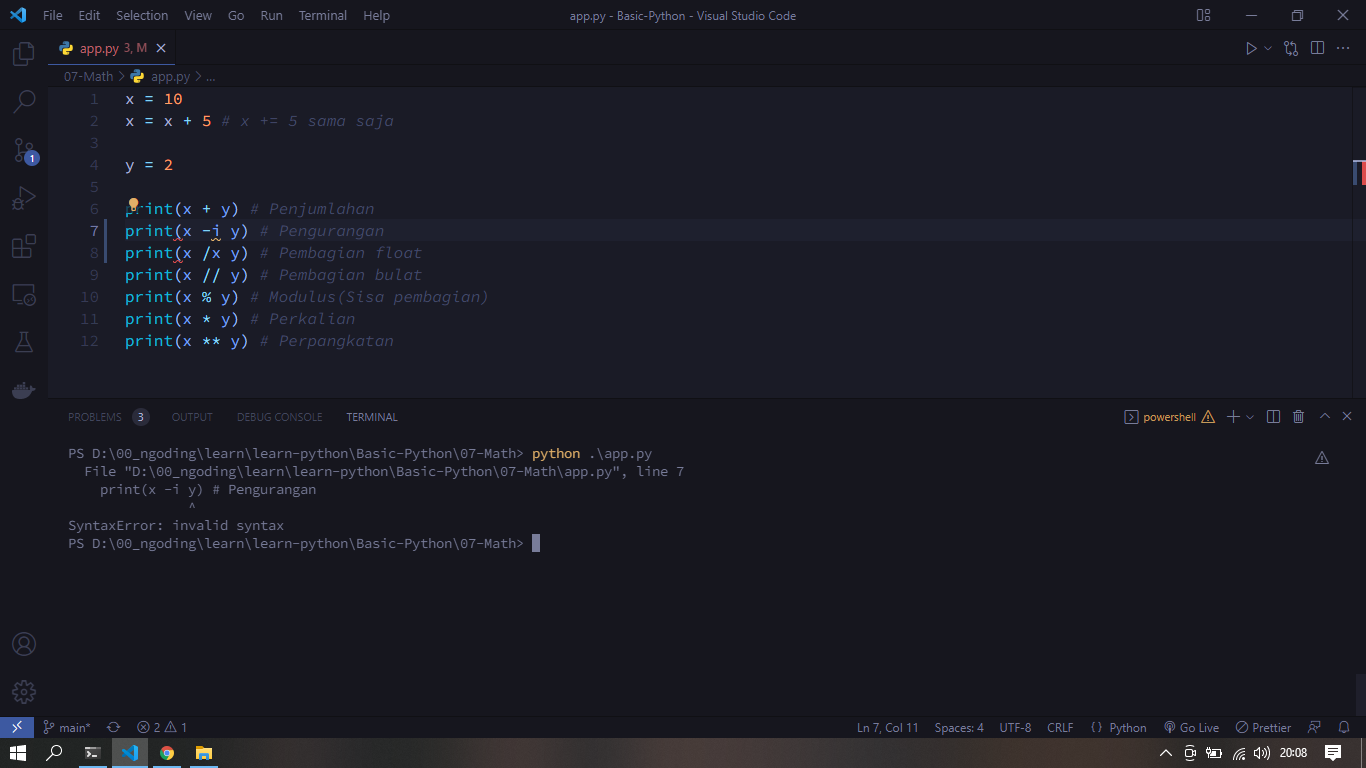
\includegraphics[width=0.5\textwidth]{gambar/08_error.png}
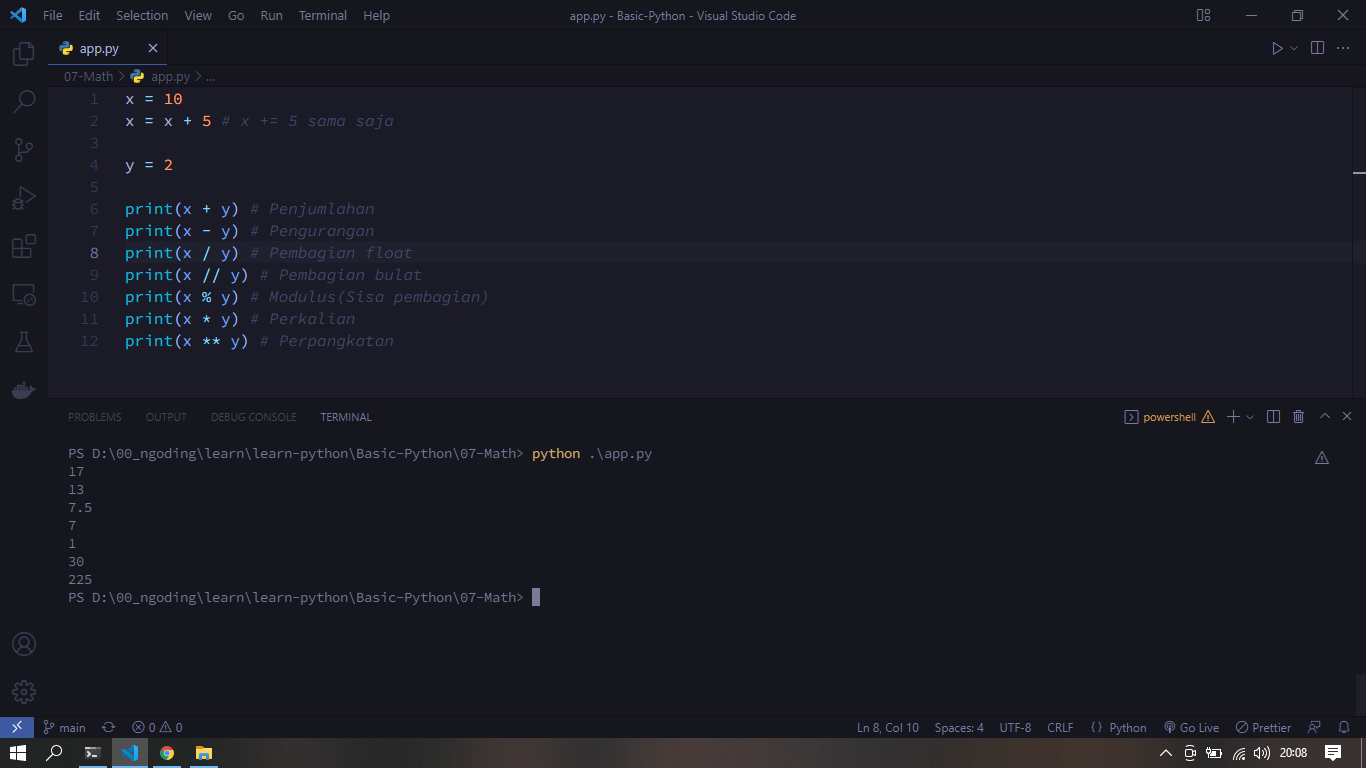
\includegraphics[width=0.5\textwidth]{gambar/08_penanganan.png}

\section{Error 20 dan penyelesaian}
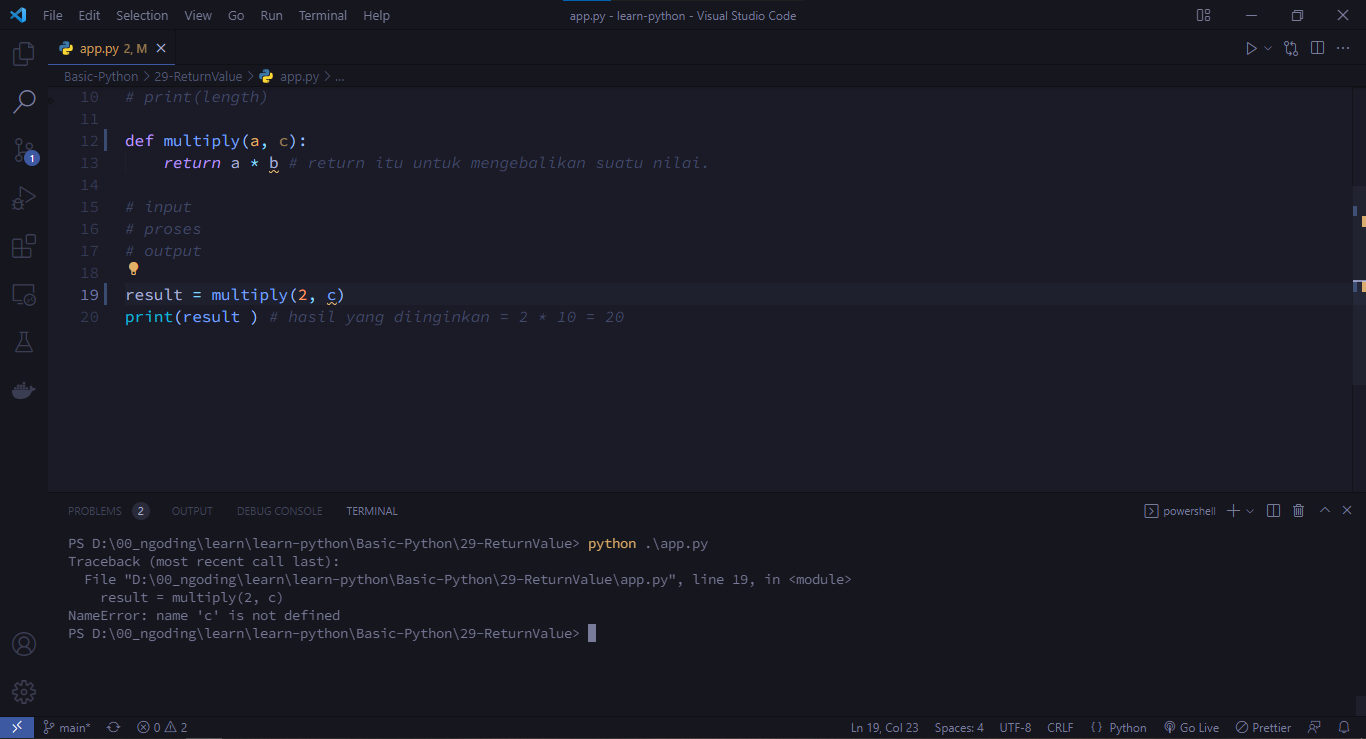
\includegraphics[width=0.5\textwidth]{gambar/29_error.png}
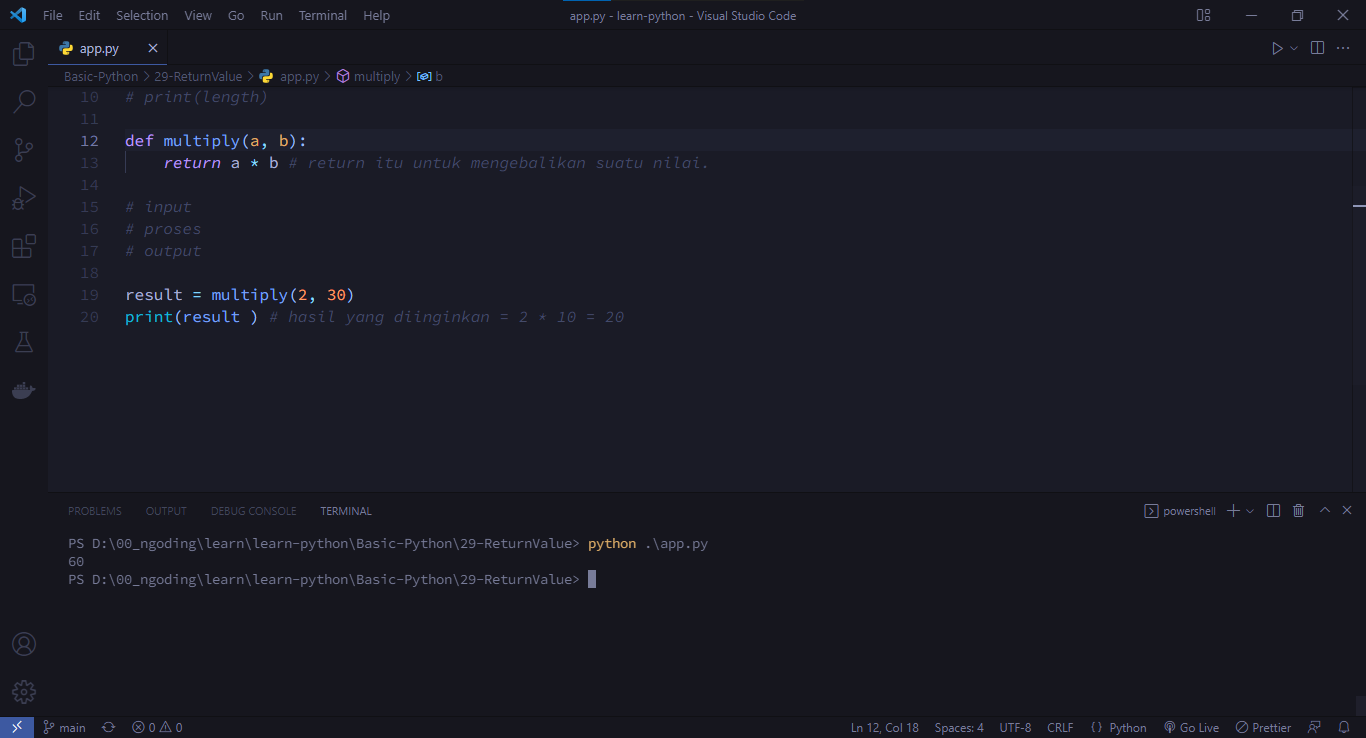
\includegraphics[width=0.5\textwidth]{gambar/29_pengananan.png}

\section{Error 21 dan penyelesaian}
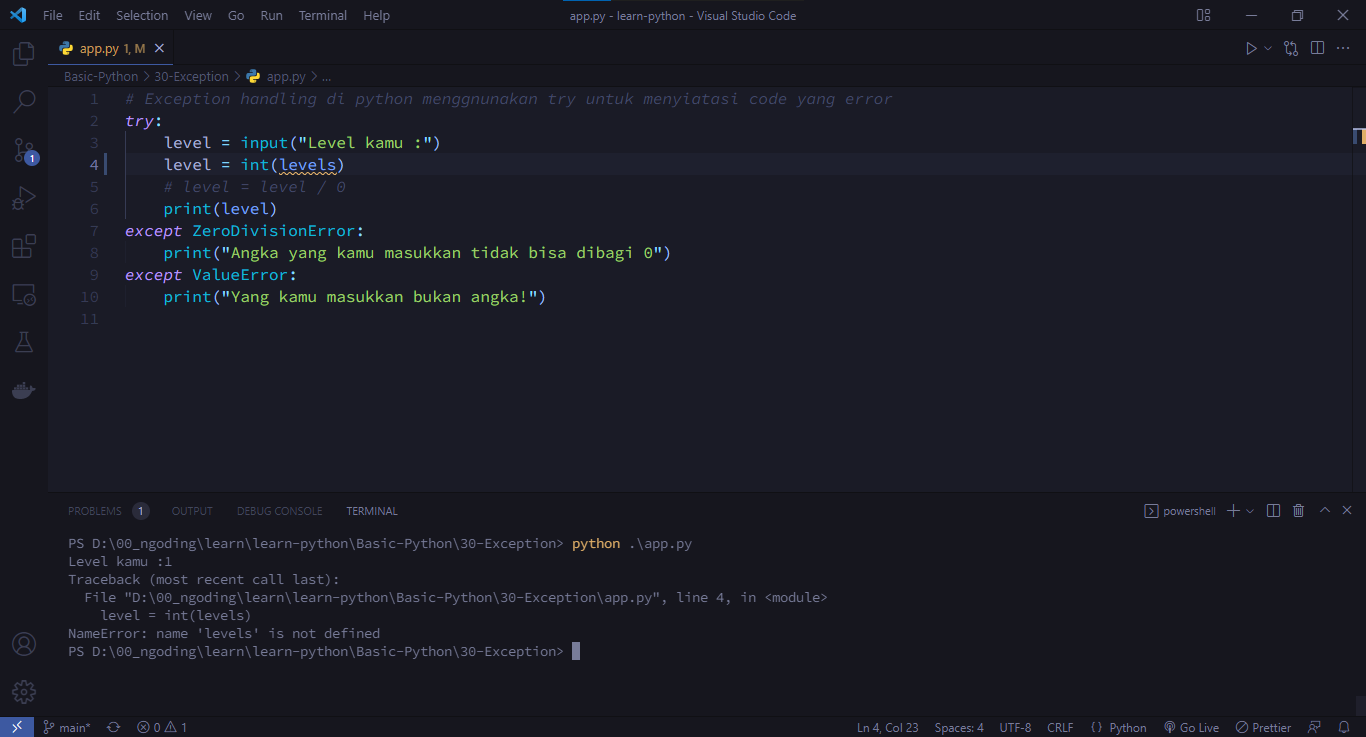
\includegraphics[width=0.5\textwidth]{gambar/30_error.png}
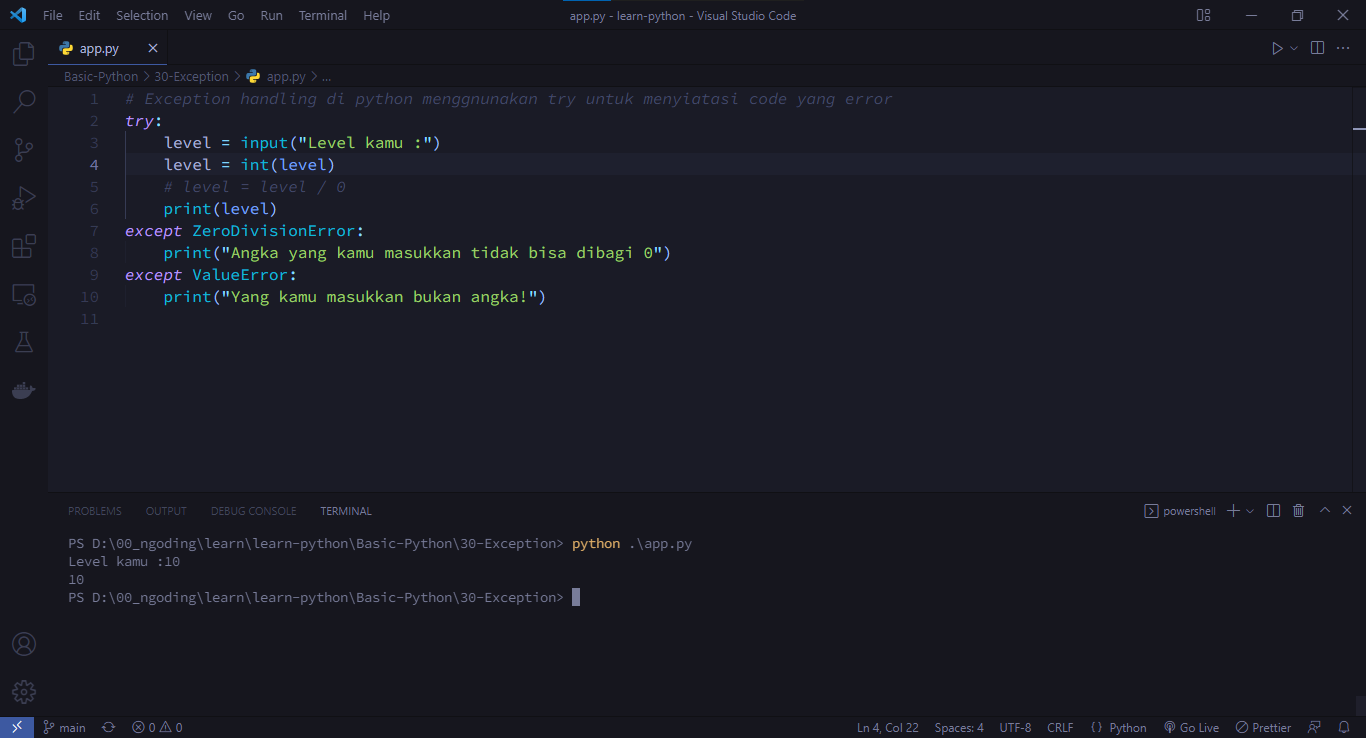
\includegraphics[width=0.5\textwidth]{gambar/30_pengananan.png}

\end{document}